\section{Available data and its quality}
\label{sec:data}

Early during the \acrshort{c19} epidemic, a surprising amount of publicly accessible data on the severity became available quickly. These data were provided by national health authorities such as the \acrfull{rki} in Germany, but also made available through aggregate data repositories, e.g. by the \acrfull{jhu} \citep{Dong2020Interactive}. These data contain information about the number of cases and deaths reported each day and depending on the data source further information, e.g., the age, sex or location of the case may be included. Here we focus on the data available for Germany, provided by the \acrshort{rki} \citep{RobertKoch-Institut2022SARSCoV2}. 

In Germany, the reporting process of these cases is regulated by law. 



\begin{figure}
    \resizebox{\textwidth}{!}{%
        % Created by tikzDevice version 0.12.6 on 2024-08-02 11:25:42
% !TEX encoding = UTF-8 Unicode
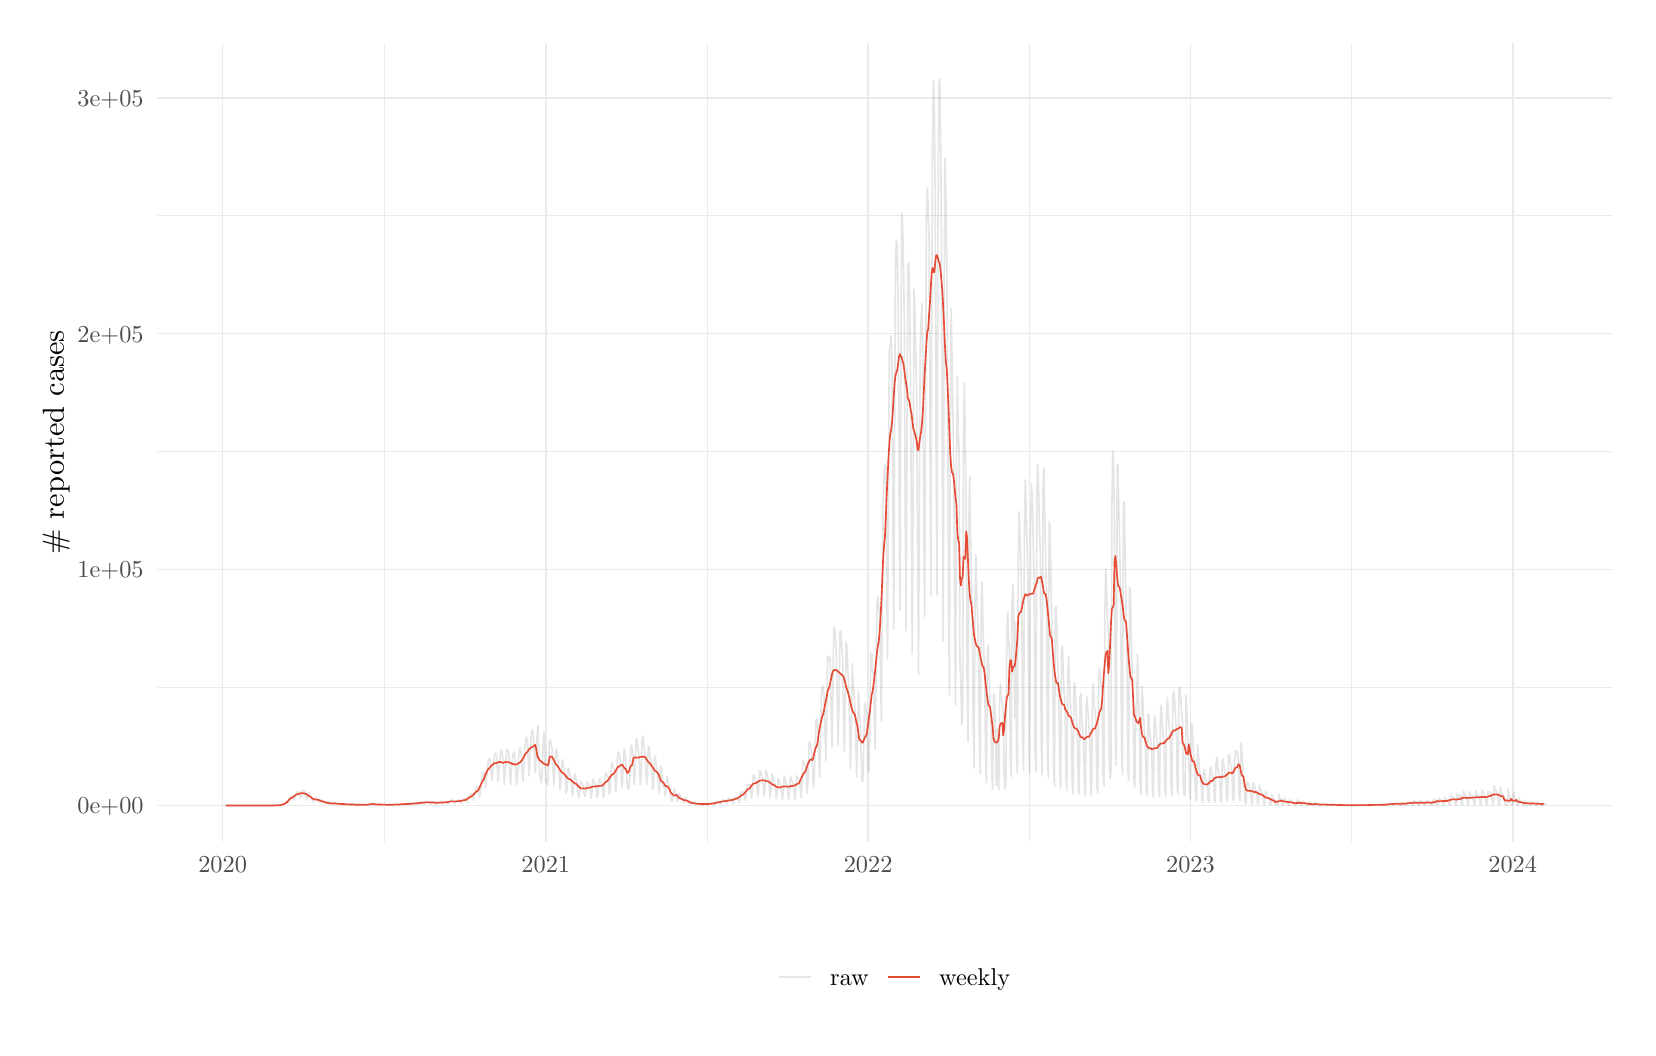
\begin{tikzpicture}[x=1pt,y=1pt]
\definecolor{fillColor}{RGB}{255,255,255}
\path[use as bounding box,fill=fillColor,fill opacity=0.00] (0,0) rectangle (578.16,361.35);
\begin{scope}
\path[clip] ( 46.86, 67.14) rectangle (572.66,355.85);
\definecolor{drawColor}{gray}{0.92}

\path[draw=drawColor,line width= 0.3pt,line join=round] ( 46.86,122.89) --
	(572.66,122.89);

\path[draw=drawColor,line width= 0.3pt,line join=round] ( 46.86,208.15) --
	(572.66,208.15);

\path[draw=drawColor,line width= 0.3pt,line join=round] ( 46.86,293.41) --
	(572.66,293.41);

\path[draw=drawColor,line width= 0.3pt,line join=round] (128.84, 67.14) --
	(128.84,355.85);

\path[draw=drawColor,line width= 0.3pt,line join=round] (245.47, 67.14) --
	(245.47,355.85);

\path[draw=drawColor,line width= 0.3pt,line join=round] (361.93, 67.14) --
	(361.93,355.85);

\path[draw=drawColor,line width= 0.3pt,line join=round] (478.40, 67.14) --
	(478.40,355.85);

\path[draw=drawColor,line width= 0.6pt,line join=round] ( 46.86, 80.26) --
	(572.66, 80.26);

\path[draw=drawColor,line width= 0.6pt,line join=round] ( 46.86,165.52) --
	(572.66,165.52);

\path[draw=drawColor,line width= 0.6pt,line join=round] ( 46.86,250.78) --
	(572.66,250.78);

\path[draw=drawColor,line width= 0.6pt,line join=round] ( 46.86,336.04) --
	(572.66,336.04);

\path[draw=drawColor,line width= 0.6pt,line join=round] ( 70.44, 67.14) --
	( 70.44,355.85);

\path[draw=drawColor,line width= 0.6pt,line join=round] (187.23, 67.14) --
	(187.23,355.85);

\path[draw=drawColor,line width= 0.6pt,line join=round] (303.70, 67.14) --
	(303.70,355.85);

\path[draw=drawColor,line width= 0.6pt,line join=round] (420.17, 67.14) --
	(420.17,355.85);

\path[draw=drawColor,line width= 0.6pt,line join=round] (536.63, 67.14) --
	(536.63,355.85);
\definecolor{drawColor}{RGB}{0,0,0}

\path[draw=drawColor,draw opacity=0.10,line width= 0.6pt,line join=round] ( 70.76, 80.26) --
	( 71.08, 80.26) --
	( 71.40, 80.26) --
	( 71.72, 80.26) --
	( 72.04, 80.26) --
	( 72.36, 80.26) --
	( 72.68, 80.26) --
	( 73.00, 80.26) --
	( 73.32, 80.26) --
	( 73.64, 80.26) --
	( 73.95, 80.26) --
	( 74.27, 80.26) --
	( 74.59, 80.26) --
	( 74.91, 80.26) --
	( 75.23, 80.26) --
	( 75.55, 80.26) --
	( 75.87, 80.26) --
	( 76.19, 80.26) --
	( 76.51, 80.26) --
	( 76.83, 80.26) --
	( 77.15, 80.26) --
	( 77.46, 80.26) --
	( 77.78, 80.26) --
	( 78.10, 80.26) --
	( 78.42, 80.26) --
	( 78.74, 80.26) --
	( 79.06, 80.26) --
	( 79.38, 80.26) --
	( 79.70, 80.26) --
	( 80.02, 80.27) --
	( 80.34, 80.26) --
	( 80.66, 80.26) --
	( 80.97, 80.26) --
	( 81.29, 80.27) --
	( 81.61, 80.26) --
	( 81.93, 80.26) --
	( 82.25, 80.26) --
	( 82.57, 80.26) --
	( 82.89, 80.26) --
	( 83.21, 80.26) --
	( 83.53, 80.26) --
	( 83.85, 80.26) --
	( 84.17, 80.26) --
	( 84.48, 80.26) --
	( 84.80, 80.26) --
	( 85.12, 80.26) --
	( 85.44, 80.26) --
	( 85.76, 80.26) --
	( 86.08, 80.26) --
	( 86.40, 80.26) --
	( 86.72, 80.26) --
	( 87.04, 80.26) --
	( 87.36, 80.26) --
	( 87.68, 80.26) --
	( 87.99, 80.27) --
	( 88.31, 80.27) --
	( 88.63, 80.28) --
	( 88.95, 80.30) --
	( 89.27, 80.28) --
	( 89.59, 80.29) --
	( 89.91, 80.30) --
	( 90.23, 80.34) --
	( 90.55, 80.40) --
	( 90.87, 80.42) --
	( 91.19, 80.42) --
	( 91.50, 80.38) --
	( 91.82, 80.35) --
	( 92.14, 80.56) --
	( 92.46, 80.77) --
	( 92.78, 80.91) --
	( 93.10, 81.11) --
	( 93.42, 81.51) --
	( 93.74, 81.37) --
	( 94.06, 81.10) --
	( 94.38, 82.00) --
	( 94.70, 82.85) --
	( 95.01, 83.34) --
	( 95.33, 83.72) --
	( 95.65, 83.72) --
	( 95.97, 83.13) --
	( 96.29, 82.19) --
	( 96.61, 83.44) --
	( 96.93, 84.42) --
	( 97.25, 85.11) --
	( 97.57, 85.30) --
	( 97.89, 85.36) --
	( 98.21, 84.29) --
	( 98.52, 82.89) --
	( 98.84, 83.79) --
	( 99.16, 85.43) --
	( 99.48, 85.60) --
	( 99.80, 85.85) --
	(100.12, 85.54) --
	(100.44, 83.96) --
	(100.76, 82.42) --
	(101.08, 83.39) --
	(101.40, 84.69) --
	(101.72, 84.77) --
	(102.03, 84.45) --
	(102.35, 83.12) --
	(102.67, 82.72) --
	(102.99, 81.86) --
	(103.31, 81.63) --
	(103.63, 82.37) --
	(103.95, 83.10) --
	(104.27, 83.18) --
	(104.59, 82.86) --
	(104.91, 82.06) --
	(105.23, 81.44) --
	(105.54, 81.72) --
	(105.86, 82.13) --
	(106.18, 82.39) --
	(106.50, 82.05) --
	(106.82, 81.89) --
	(107.14, 81.35) --
	(107.46, 80.86) --
	(107.78, 81.21) --
	(108.10, 81.52) --
	(108.42, 81.48) --
	(108.74, 81.51) --
	(109.05, 81.05) --
	(109.37, 80.79) --
	(109.69, 80.62) --
	(110.01, 80.88) --
	(110.33, 81.20) --
	(110.65, 81.30) --
	(110.97, 81.29) --
	(111.29, 81.10) --
	(111.61, 80.84) --
	(111.93, 80.55) --
	(112.25, 80.85) --
	(112.56, 80.99) --
	(112.88, 81.04) --
	(113.20, 80.96) --
	(113.52, 80.89) --
	(113.84, 80.66) --
	(114.16, 80.53) --
	(114.48, 80.72) --
	(114.80, 80.89) --
	(115.12, 80.97) --
	(115.44, 80.62) --
	(115.76, 80.71) --
	(116.07, 80.55) --
	(116.39, 80.45) --
	(116.71, 80.61) --
	(117.03, 80.79) --
	(117.35, 80.82) --
	(117.67, 80.71) --
	(117.99, 80.64) --
	(118.31, 80.58) --
	(118.63, 80.41) --
	(118.95, 80.38) --
	(119.27, 80.52) --
	(119.58, 80.69) --
	(119.90, 80.71) --
	(120.22, 80.63) --
	(120.54, 80.51) --
	(120.86, 80.40) --
	(121.18, 80.51) --
	(121.50, 80.63) --
	(121.82, 80.70) --
	(122.14, 80.50) --
	(122.46, 80.56) --
	(122.78, 80.52) --
	(123.09, 80.41) --
	(123.41, 80.48) --
	(123.73, 80.70) --
	(124.05, 81.00) --
	(124.37, 80.92) --
	(124.69, 81.11) --
	(125.01, 80.75) --
	(125.33, 80.45) --
	(125.65, 80.64) --
	(125.97, 80.72) --
	(126.29, 80.70) --
	(126.60, 80.75) --
	(126.92, 80.75) --
	(127.24, 80.54) --
	(127.56, 80.43) --
	(127.88, 80.62) --
	(128.20, 80.65) --
	(128.52, 80.67) --
	(128.84, 80.66) --
	(129.16, 80.63) --
	(129.48, 80.51) --
	(129.80, 80.39) --
	(130.11, 80.54) --
	(130.43, 80.60) --
	(130.75, 80.65) --
	(131.07, 80.62) --
	(131.39, 80.63) --
	(131.71, 80.50) --
	(132.03, 80.38) --
	(132.35, 80.54) --
	(132.67, 80.66) --
	(132.99, 80.73) --
	(133.31, 80.74) --
	(133.62, 80.71) --
	(133.94, 80.64) --
	(134.26, 80.42) --
	(134.58, 80.65) --
	(134.90, 80.71) --
	(135.22, 80.86) --
	(135.54, 80.85) --
	(135.86, 80.95) --
	(136.18, 80.73) --
	(136.50, 80.44) --
	(136.82, 80.71) --
	(137.13, 80.91) --
	(137.45, 81.04) --
	(137.77, 81.00) --
	(138.09, 81.04) --
	(138.41, 80.74) --
	(138.73, 80.52) --
	(139.05, 80.94) --
	(139.37, 81.07) --
	(139.69, 81.21) --
	(140.01, 81.26) --
	(140.33, 81.12) --
	(140.64, 80.87) --
	(140.96, 80.53) --
	(141.28, 81.20) --
	(141.60, 81.28) --
	(141.92, 81.58) --
	(142.24, 81.55) --
	(142.56, 81.44) --
	(142.88, 80.91) --
	(143.20, 80.68) --
	(143.52, 81.58) --
	(143.84, 81.57) --
	(144.15, 81.76) --
	(144.47, 81.64) --
	(144.79, 81.68) --
	(145.11, 81.05) --
	(145.43, 80.74) --
	(145.75, 81.48) --
	(146.07, 81.53) --
	(146.39, 81.65) --
	(146.71, 81.58) --
	(147.03, 81.45) --
	(147.35, 80.97) --
	(147.66, 80.72) --
	(147.98, 81.27) --
	(148.30, 81.39) --
	(148.62, 81.47) --
	(148.94, 81.55) --
	(149.26, 81.54) --
	(149.58, 81.21) --
	(149.90, 80.76) --
	(150.22, 81.47) --
	(150.54, 81.44) --
	(150.86, 81.75) --
	(151.17, 81.62) --
	(151.49, 81.68) --
	(151.81, 81.31) --
	(152.13, 80.91) --
	(152.45, 81.53) --
	(152.77, 81.97) --
	(153.09, 82.12) --
	(153.41, 82.28) --
	(153.73, 82.11) --
	(154.05, 81.45) --
	(154.37, 80.85) --
	(154.68, 81.67) --
	(155.00, 81.81) --
	(155.32, 82.15) --
	(155.64, 82.30) --
	(155.96, 82.25) --
	(156.28, 81.78) --
	(156.60, 81.01) --
	(156.92, 81.83) --
	(157.24, 82.11) --
	(157.56, 82.60) --
	(157.88, 82.76) --
	(158.19, 82.76) --
	(158.51, 82.14) --
	(158.83, 81.25) --
	(159.15, 82.32) --
	(159.47, 83.32) --
	(159.79, 84.10) --
	(160.11, 84.25) --
	(160.43, 84.58) --
	(160.75, 83.35) --
	(161.07, 82.20) --
	(161.39, 83.84) --
	(161.70, 84.84) --
	(162.02, 86.44) --
	(162.34, 87.00) --
	(162.66, 87.06) --
	(162.98, 85.10) --
	(163.30, 83.40) --
	(163.62, 85.77) --
	(163.94, 88.31) --
	(164.26, 90.84) --
	(164.58, 92.12) --
	(164.90, 92.24) --
	(165.21, 89.72) --
	(165.53, 86.62) --
	(165.85, 90.52) --
	(166.17, 93.86) --
	(166.49, 96.67) --
	(166.81, 97.18) --
	(167.13, 96.81) --
	(167.45, 92.19) --
	(167.77, 89.25) --
	(168.09, 93.26) --
	(168.41, 96.75) --
	(168.72, 98.34) --
	(169.04, 99.26) --
	(169.36, 98.65) --
	(169.68, 93.84) --
	(170.00, 88.90) --
	(170.32, 93.90) --
	(170.64, 96.99) --
	(170.96, 99.63) --
	(171.28,100.35) --
	(171.60, 98.44) --
	(171.92, 93.74) --
	(172.23, 87.81) --
	(172.55, 92.80) --
	(172.87, 97.64) --
	(173.19,100.45) --
	(173.51,100.52) --
	(173.83, 99.29) --
	(174.15, 92.85) --
	(174.47, 87.77) --
	(174.79, 93.11) --
	(175.11, 96.81) --
	(175.43, 99.04) --
	(175.74, 99.65) --
	(176.06, 97.45) --
	(176.38, 93.00) --
	(176.70, 87.75) --
	(177.02, 91.60) --
	(177.34, 96.69) --
	(177.66,100.04) --
	(177.98,101.11) --
	(178.30, 99.16) --
	(178.62, 93.66) --
	(178.94, 88.98) --
	(179.25, 94.26) --
	(179.57, 99.72) --
	(179.89,103.81) --
	(180.21,105.01) --
	(180.53,103.50) --
	(180.85, 97.85) --
	(181.17, 90.92) --
	(181.49, 96.47) --
	(181.81,103.20) --
	(182.13,107.01) --
	(182.45,107.51) --
	(182.76,105.58) --
	(183.08, 98.79) --
	(183.40, 92.13) --
	(183.72, 97.55) --
	(184.04,104.94) --
	(184.36,109.20) --
	(184.68, 98.27) --
	(185.00, 91.47) --
	(185.32, 90.11) --
	(185.64, 88.63) --
	(185.96, 93.65) --
	(186.27,103.75) --
	(186.59,106.74) --
	(186.91, 96.94) --
	(187.23, 89.00) --
	(187.55, 88.79) --
	(187.87, 87.79) --
	(188.19, 92.50) --
	(188.51,103.64) --
	(188.83,104.08) --
	(189.15,102.51) --
	(189.47,101.19) --
	(189.78, 94.47) --
	(190.10, 87.48) --
	(190.42, 91.77) --
	(190.74, 99.52) --
	(191.06,100.82) --
	(191.38, 97.65) --
	(191.70, 95.87) --
	(192.02, 91.71) --
	(192.34, 85.88) --
	(192.66, 88.08) --
	(192.98, 96.01) --
	(193.29, 96.86) --
	(193.61, 94.61) --
	(193.93, 93.08) --
	(194.25, 90.13) --
	(194.57, 84.54) --
	(194.89, 86.02) --
	(195.21, 93.49) --
	(195.53, 93.75) --
	(195.85, 91.65) --
	(196.17, 90.98) --
	(196.49, 88.75) --
	(196.80, 83.85) --
	(197.12, 85.26) --
	(197.44, 90.75) --
	(197.76, 91.71) --
	(198.08, 90.08) --
	(198.40, 88.81) --
	(198.72, 87.41) --
	(199.04, 82.90) --
	(199.36, 83.84) --
	(199.68, 88.01) --
	(200.00, 89.03) --
	(200.31, 88.25) --
	(200.63, 87.54) --
	(200.95, 85.03) --
	(201.27, 83.47) --
	(201.59, 84.01) --
	(201.91, 88.13) --
	(202.23, 88.78) --
	(202.55, 88.12) --
	(202.87, 87.69) --
	(203.19, 86.89) --
	(203.51, 82.84) --
	(203.82, 84.02) --
	(204.14, 88.93) --
	(204.46, 89.90) --
	(204.78, 88.70) --
	(205.10, 88.34) --
	(205.42, 86.79) --
	(205.74, 83.21) --
	(206.06, 84.26) --
	(206.38, 89.61) --
	(206.70, 89.91) --
	(207.02, 88.90) --
	(207.33, 88.49) --
	(207.65, 87.34) --
	(207.97, 83.13) --
	(208.29, 84.40) --
	(208.61, 90.08) --
	(208.93, 92.20) --
	(209.25, 91.48) --
	(209.57, 90.97) --
	(209.89, 89.19) --
	(210.21, 84.39) --
	(210.53, 86.10) --
	(210.84, 93.72) --
	(211.16, 95.92) --
	(211.48, 94.53) --
	(211.80, 93.65) --
	(212.12, 91.53) --
	(212.44, 85.34) --
	(212.76, 87.85) --
	(213.08, 96.85) --
	(213.40, 99.56) --
	(213.72, 98.94) --
	(214.04, 97.35) --
	(214.35, 93.72) --
	(214.67, 86.73) --
	(214.99, 89.64) --
	(215.31, 97.64) --
	(215.63,100.71) --
	(215.95, 98.52) --
	(216.27, 93.46) --
	(216.59, 89.30) --
	(216.91, 86.35) --
	(217.23, 86.25) --
	(217.55, 90.07) --
	(217.86,100.49) --
	(218.18,102.22) --
	(218.50,100.12) --
	(218.82, 95.66) --
	(219.14, 87.81) --
	(219.46, 90.59) --
	(219.78,103.05) --
	(220.10,104.61) --
	(220.42,101.63) --
	(220.74, 99.94) --
	(221.06, 95.34) --
	(221.37, 87.77) --
	(221.69, 90.75) --
	(222.01,104.10) --
	(222.33,105.30) --
	(222.65,101.94) --
	(222.97, 99.84) --
	(223.29, 95.61) --
	(223.61, 87.65) --
	(223.93, 90.65) --
	(224.25,101.79) --
	(224.57,101.58) --
	(224.88, 98.51) --
	(225.20, 96.59) --
	(225.52, 93.09) --
	(225.84, 85.93) --
	(226.16, 88.03) --
	(226.48, 98.14) --
	(226.80, 98.03) --
	(227.12, 94.88) --
	(227.44, 93.44) --
	(227.76, 90.50) --
	(228.08, 84.80) --
	(228.39, 86.56) --
	(228.71, 94.54) --
	(229.03, 94.30) --
	(229.35, 88.50) --
	(229.67, 86.77) --
	(229.99, 87.59) --
	(230.31, 83.90) --
	(230.63, 84.73) --
	(230.95, 90.76) --
	(231.27, 89.90) --
	(231.59, 87.44) --
	(231.90, 86.72) --
	(232.22, 85.23) --
	(232.54, 81.97) --
	(232.86, 81.80) --
	(233.18, 83.39) --
	(233.50, 86.35) --
	(233.82, 86.05) --
	(234.14, 84.67) --
	(234.46, 83.41) --
	(234.78, 81.63) --
	(235.10, 82.34) --
	(235.41, 84.61) --
	(235.73, 84.09) --
	(236.05, 82.76) --
	(236.37, 82.20) --
	(236.69, 82.23) --
	(237.01, 81.23) --
	(237.33, 81.73) --
	(237.65, 83.28) --
	(237.97, 82.70) --
	(238.29, 82.21) --
	(238.61, 81.83) --
	(238.92, 81.38) --
	(239.24, 80.70) --
	(239.56, 81.06) --
	(239.88, 81.71) --
	(240.20, 81.49) --
	(240.52, 81.25) --
	(240.84, 81.14) --
	(241.16, 80.89) --
	(241.48, 80.50) --
	(241.80, 80.78) --
	(242.12, 81.17) --
	(242.43, 81.03) --
	(242.75, 80.97) --
	(243.07, 80.89) --
	(243.39, 80.67) --
	(243.71, 80.45) --
	(244.03, 80.71) --
	(244.35, 81.03) --
	(244.67, 81.00) --
	(244.99, 80.87) --
	(245.31, 80.83) --
	(245.63, 80.70) --
	(245.94, 80.44) --
	(246.26, 80.74) --
	(246.58, 81.17) --
	(246.90, 81.08) --
	(247.22, 81.08) --
	(247.54, 81.07) --
	(247.86, 80.94) --
	(248.18, 80.53) --
	(248.50, 80.95) --
	(248.82, 81.77) --
	(249.14, 81.65) --
	(249.45, 81.56) --
	(249.77, 81.64) --
	(250.09, 81.36) --
	(250.41, 80.69) --
	(250.73, 81.48) --
	(251.05, 82.26) --
	(251.37, 82.22) --
	(251.69, 82.16) --
	(252.01, 82.07) --
	(252.33, 81.62) --
	(252.65, 80.81) --
	(252.96, 81.68) --
	(253.28, 82.90) --
	(253.60, 82.69) --
	(253.92, 82.51) --
	(254.24, 82.42) --
	(254.56, 81.94) --
	(254.88, 80.93) --
	(255.20, 82.07) --
	(255.52, 83.47) --
	(255.84, 83.28) --
	(256.16, 83.27) --
	(256.47, 83.28) --
	(256.79, 82.64) --
	(257.11, 81.24) --
	(257.43, 82.76) --
	(257.75, 85.01) --
	(258.07, 85.08) --
	(258.39, 84.91) --
	(258.71, 85.20) --
	(259.03, 84.22) --
	(259.35, 82.03) --
	(259.67, 84.12) --
	(259.98, 87.87) --
	(260.30, 87.73) --
	(260.62, 87.67) --
	(260.94, 87.80) --
	(261.26, 86.08) --
	(261.58, 82.90) --
	(261.90, 85.87) --
	(262.22, 91.26) --
	(262.54, 91.11) --
	(262.86, 90.18) --
	(263.17, 89.13) --
	(263.49, 87.43) --
	(263.81, 83.45) --
	(264.13, 86.31) --
	(264.45, 92.69) --
	(264.77, 92.83) --
	(265.09, 91.11) --
	(265.41, 90.56) --
	(265.73, 88.34) --
	(266.05, 83.71) --
	(266.37, 86.24) --
	(266.68, 93.15) --
	(267.00, 92.33) --
	(267.32, 90.83) --
	(267.64, 89.76) --
	(267.96, 87.56) --
	(268.28, 83.06) --
	(268.60, 86.13) --
	(268.92, 91.68) --
	(269.24, 90.69) --
	(269.56, 89.02) --
	(269.88, 87.84) --
	(270.19, 86.26) --
	(270.51, 82.63) --
	(270.83, 84.88) --
	(271.15, 89.86) --
	(271.47, 89.18) --
	(271.79, 88.01) --
	(272.11, 87.44) --
	(272.43, 85.68) --
	(272.75, 82.52) --
	(273.07, 85.18) --
	(273.39, 91.05) --
	(273.70, 89.96) --
	(274.02, 88.36) --
	(274.34, 87.42) --
	(274.66, 85.51) --
	(274.98, 82.52) --
	(275.30, 85.10) --
	(275.62, 90.68) --
	(275.94, 89.74) --
	(276.26, 88.91) --
	(276.58, 88.12) --
	(276.90, 86.25) --
	(277.21, 82.51) --
	(277.53, 85.60) --
	(277.85, 91.04) --
	(278.17, 90.55) --
	(278.49, 89.93) --
	(278.81, 89.77) --
	(279.13, 87.50) --
	(279.45, 83.17) --
	(279.77, 87.20) --
	(280.09, 96.60) --
	(280.41, 95.59) --
	(280.72, 95.01) --
	(281.04, 94.48) --
	(281.36, 91.59) --
	(281.68, 84.68) --
	(282.00, 90.38) --
	(282.32,102.76) --
	(282.64,103.54) --
	(282.96,101.02) --
	(283.28, 99.50) --
	(283.60, 94.82) --
	(283.92, 86.62) --
	(284.23, 90.05) --
	(284.55,101.07) --
	(284.87,111.08) --
	(285.19,111.36) --
	(285.51,109.03) --
	(285.83,100.53) --
	(286.15, 90.37) --
	(286.47,100.98) --
	(286.79,120.50) --
	(287.11,123.62) --
	(287.43,122.67) --
	(287.74,119.55) --
	(288.06,109.23) --
	(288.38, 96.49) --
	(288.70,109.75) --
	(289.02,133.98) --
	(289.34,134.14) --
	(289.66,132.46) --
	(289.98,133.59) --
	(290.30,116.35) --
	(290.62,101.39) --
	(290.94,120.05) --
	(291.25,143.82) --
	(291.57,144.82) --
	(291.89,141.53) --
	(292.21,134.90) --
	(292.53,118.57) --
	(292.85,102.04) --
	(293.17,118.07) --
	(293.49,143.02) --
	(293.81,143.37) --
	(294.13,138.24) --
	(294.45,133.57) --
	(294.76,116.48) --
	(295.08, 99.93) --
	(295.40,116.51) --
	(295.72,139.38) --
	(296.04,137.56) --
	(296.36,129.43) --
	(296.68,123.86) --
	(297.00,109.78) --
	(297.32, 93.51) --
	(297.64,107.20) --
	(297.96,131.59) --
	(298.27,124.96) --
	(298.59,120.56) --
	(298.91,115.44) --
	(299.23,104.58) --
	(299.55, 90.69) --
	(299.87,103.25) --
	(300.19,121.40) --
	(300.51,115.15) --
	(300.83,110.09) --
	(301.15, 98.93) --
	(301.47, 89.15) --
	(301.78, 89.14) --
	(302.10,101.13) --
	(302.42,117.22) --
	(302.74,115.77) --
	(303.06,115.61) --
	(303.38,104.96) --
	(303.70, 92.39) --
	(304.02, 92.69) --
	(304.34,110.92) --
	(304.66,135.29) --
	(304.98,135.24) --
	(305.29,128.25) --
	(305.61,127.91) --
	(305.93,111.85) --
	(306.25,100.51) --
	(306.57,126.06) --
	(306.89,153.68) --
	(307.21,155.64) --
	(307.53,151.95) --
	(307.85,149.14) --
	(308.17,129.16) --
	(308.49,110.63) --
	(308.80,150.81) --
	(309.12,188.35) --
	(309.44,199.79) --
	(309.76,203.56) --
	(310.08,203.18) --
	(310.40,162.40) --
	(310.72,133.10) --
	(311.04,199.09) --
	(311.36,245.23) --
	(311.68,246.39) --
	(312.00,250.05) --
	(312.31,240.47) --
	(312.63,186.72) --
	(312.95,144.08) --
	(313.27,216.01) --
	(313.59,277.11) --
	(313.91,284.48) --
	(314.23,282.41) --
	(314.55,259.14) --
	(314.87,193.93) --
	(315.19,150.95) --
	(315.51,232.17) --
	(315.82,294.25) --
	(316.14,291.23) --
	(316.46,276.44) --
	(316.78,256.46) --
	(317.10,184.72) --
	(317.42,143.56) --
	(317.74,215.66) --
	(318.06,275.43) --
	(318.38,276.50) --
	(318.70,262.11) --
	(319.02,232.91) --
	(319.33,182.50) --
	(319.65,135.05) --
	(319.97,199.39) --
	(320.29,266.81) --
	(320.61,257.84) --
	(320.93,242.29) --
	(321.25,226.76) --
	(321.57,173.03) --
	(321.89,127.58) --
	(322.21,190.06) --
	(322.53,245.62) --
	(322.84,255.51) --
	(323.16,261.67) --
	(323.48,242.40) --
	(323.80,184.69) --
	(324.12,148.39) --
	(324.44,221.77) --
	(324.76,291.63) --
	(325.08,303.32) --
	(325.40,297.22) --
	(325.72,283.83) --
	(326.04,213.29) --
	(326.35,156.20) --
	(326.67,257.57) --
	(326.99,323.35) --
	(327.31,342.30) --
	(327.63,331.63) --
	(327.95,297.46) --
	(328.27,202.42) --
	(328.59,156.43) --
	(328.91,282.96) --
	(329.23,340.23) --
	(329.55,342.73) --
	(329.86,324.23) --
	(330.18,288.47) --
	(330.50,198.21) --
	(330.82,139.71) --
	(331.14,256.65) --
	(331.46,314.19) --
	(331.78,301.87) --
	(332.10,278.08) --
	(332.42,235.46) --
	(332.74,159.67) --
	(333.06,119.99) --
	(333.37,212.69) --
	(333.69,260.01) --
	(334.01,241.35) --
	(334.33,223.26) --
	(334.65,202.07) --
	(334.97,145.16) --
	(335.29,116.70) --
	(335.61,199.92) --
	(335.93,235.58) --
	(336.25,215.75) --
	(336.57,208.64) --
	(336.88,132.23) --
	(337.20,124.59) --
	(337.52,109.45) --
	(337.84,111.75) --
	(338.16,215.54) --
	(338.48,233.26) --
	(338.80,213.00) --
	(339.12,182.13) --
	(339.44,126.68) --
	(339.76,103.27) --
	(340.08,181.57) --
	(340.39,199.08) --
	(340.71,178.70) --
	(341.03,160.98) --
	(341.35,146.99) --
	(341.67,109.25) --
	(341.99, 93.78) --
	(342.31,154.02) --
	(342.63,171.05) --
	(342.95,156.86) --
	(343.27,148.78) --
	(343.59,137.52) --
	(343.90,103.27) --
	(344.22, 91.65) --
	(344.54,152.58) --
	(344.86,161.12) --
	(345.18,146.04) --
	(345.50,135.64) --
	(345.82,128.78) --
	(346.14, 97.41) --
	(346.46, 88.49) --
	(346.78,136.23) --
	(347.10,138.30) --
	(347.41,126.12) --
	(347.73,118.00) --
	(348.05,114.32) --
	(348.37, 92.04) --
	(348.69, 86.18) --
	(349.01,120.39) --
	(349.33,120.06) --
	(349.65,110.42) --
	(349.97, 87.37) --
	(350.29,108.06) --
	(350.61, 89.32) --
	(350.92, 85.77) --
	(351.24,120.24) --
	(351.56,124.19) --
	(351.88,118.58) --
	(352.20,116.42) --
	(352.52,113.89) --
	(352.84, 91.15) --
	(353.16, 86.34) --
	(353.48, 88.26) --
	(353.80,141.05) --
	(354.12,150.24) --
	(354.43,141.04) --
	(354.75,135.93) --
	(355.07, 97.12) --
	(355.39, 90.76) --
	(355.71,154.47) --
	(356.03,160.05) --
	(356.35,150.07) --
	(356.67,112.05) --
	(356.99,146.38) --
	(357.31,100.01) --
	(357.63, 91.60) --
	(357.94,170.26) --
	(358.26,186.47) --
	(358.58,177.05) --
	(358.90,166.69) --
	(359.22,154.60) --
	(359.54,103.46) --
	(359.86, 92.88) --
	(360.18,179.93) --
	(360.50,197.99) --
	(360.82,186.93) --
	(361.14,174.27) --
	(361.45,161.14) --
	(361.77,100.65) --
	(362.09, 91.84) --
	(362.41,183.23) --
	(362.73,196.71) --
	(363.05,188.91) --
	(363.37,174.78) --
	(363.69,161.77) --
	(364.01,100.42) --
	(364.33, 92.51) --
	(364.65,191.92) --
	(364.96,203.54) --
	(365.28,195.86) --
	(365.60,179.95) --
	(365.92,172.87) --
	(366.24,101.85) --
	(366.56, 91.46) --
	(366.88,194.81) --
	(367.20,202.48) --
	(367.52,184.36) --
	(367.84,168.65) --
	(368.16,156.56) --
	(368.47, 99.24) --
	(368.79, 90.47) --
	(369.11,182.76) --
	(369.43,180.93) --
	(369.75,162.21) --
	(370.07,144.60) --
	(370.39,133.22) --
	(370.71, 93.67) --
	(371.03, 87.11) --
	(371.35,151.97) --
	(371.67,152.19) --
	(371.98,138.99) --
	(372.30,128.21) --
	(372.62,121.77) --
	(372.94, 91.74) --
	(373.26, 86.41) --
	(373.58,136.68) --
	(373.90,137.82) --
	(374.22,127.96) --
	(374.54,120.68) --
	(374.86,117.39) --
	(375.18, 89.80) --
	(375.49, 85.84) --
	(375.81,126.68) --
	(376.13,134.06) --
	(376.45,124.94) --
	(376.77,116.83) --
	(377.09,110.67) --
	(377.41, 88.55) --
	(377.73, 84.62) --
	(378.05,123.27) --
	(378.37,124.67) --
	(378.69,117.91) --
	(379.00,110.85) --
	(379.32,107.88) --
	(379.64, 87.20) --
	(379.96, 84.44) --
	(380.28,119.61) --
	(380.60,120.76) --
	(380.92,111.70) --
	(381.24,106.20) --
	(381.56,104.76) --
	(381.88, 87.01) --
	(382.20, 83.81) --
	(382.51,116.83) --
	(382.83,119.40) --
	(383.15,113.88) --
	(383.47,108.96) --
	(383.79,106.10) --
	(384.11, 86.70) --
	(384.43, 83.98) --
	(384.75,120.46) --
	(385.07,124.26) --
	(385.39,116.81) --
	(385.71,113.78) --
	(386.02,110.07) --
	(386.34, 87.18) --
	(386.66, 84.45) --
	(386.98,127.06) --
	(387.30,129.99) --
	(387.62,126.14) --
	(387.94,122.43) --
	(388.26,121.30) --
	(388.58, 91.90) --
	(388.90, 87.33) --
	(389.22,149.48) --
	(389.53,165.66) --
	(389.85,159.04) --
	(390.17,147.16) --
	(390.49,143.51) --
	(390.81, 98.11) --
	(391.13, 90.08) --
	(391.45, 92.71) --
	(391.77,188.71) --
	(392.09,208.44) --
	(392.41,201.97) --
	(392.73,178.78) --
	(393.04,102.99) --
	(393.36, 94.76) --
	(393.68,203.57) --
	(394.00,202.61) --
	(394.32,186.34) --
	(394.64,170.82) --
	(394.96,157.98) --
	(395.28, 99.25) --
	(395.60, 91.58) --
	(395.92,188.63) --
	(396.24,190.09) --
	(396.55,171.26) --
	(396.87,152.56) --
	(397.19,140.22) --
	(397.51, 94.76) --
	(397.83, 89.29) --
	(398.15,159.06) --
	(398.47,158.10) --
	(398.79,139.80) --
	(399.11,128.17) --
	(399.43,119.32) --
	(399.75, 89.32) --
	(400.06, 86.85) --
	(400.38,115.78) --
	(400.70,112.68) --
	(401.02,135.08) --
	(401.34,121.91) --
	(401.66,112.34) --
	(401.98, 87.42) --
	(402.30, 84.30) --
	(402.62,123.33) --
	(402.94,119.22) --
	(403.26,111.74) --
	(403.57,106.73) --
	(403.89,103.53) --
	(404.21, 85.49) --
	(404.53, 84.03) --
	(404.85,113.48) --
	(405.17,112.64) --
	(405.49,106.18) --
	(405.81,103.25) --
	(406.13,102.24) --
	(406.45, 85.43) --
	(406.77, 83.28) --
	(407.08,111.40) --
	(407.40,112.63) --
	(407.72,107.40) --
	(408.04,104.11) --
	(408.36,102.58) --
	(408.68, 85.76) --
	(409.00, 83.40) --
	(409.32,113.89) --
	(409.64,116.52) --
	(409.96,109.97) --
	(410.28,105.63) --
	(410.59,103.87) --
	(410.91, 85.89) --
	(411.23, 83.65) --
	(411.55,114.05) --
	(411.87,119.30) --
	(412.19,112.51) --
	(412.51,108.64) --
	(412.83,106.09) --
	(413.15, 87.45) --
	(413.47, 83.90) --
	(413.79,119.54) --
	(414.10,121.85) --
	(414.42,118.60) --
	(414.74,112.58) --
	(415.06,107.78) --
	(415.38, 87.26) --
	(415.70, 84.32) --
	(416.02,122.14) --
	(416.34,123.28) --
	(416.66,118.67) --
	(416.98,114.47) --
	(417.30,109.79) --
	(417.61, 86.97) --
	(417.93, 83.97) --
	(418.25, 84.25) --
	(418.57,120.14) --
	(418.89,114.19) --
	(419.21,105.80) --
	(419.53, 99.85) --
	(419.85, 84.42) --
	(420.17, 82.42) --
	(420.49,110.08) --
	(420.81,108.66) --
	(421.12,101.33) --
	(421.44, 97.33) --
	(421.76, 90.96) --
	(422.08, 82.87) --
	(422.40, 81.72) --
	(422.72,102.19) --
	(423.04, 98.91) --
	(423.36, 94.22) --
	(423.68, 90.35) --
	(424.00, 88.55) --
	(424.32, 82.21) --
	(424.63, 81.38) --
	(424.95, 93.39) --
	(425.27, 92.55) --
	(425.59, 89.86) --
	(425.91, 88.58) --
	(426.23, 87.70) --
	(426.55, 82.00) --
	(426.87, 81.37) --
	(427.19, 93.09) --
	(427.51, 94.39) --
	(427.83, 92.12) --
	(428.14, 91.16) --
	(428.46, 89.74) --
	(428.78, 82.21) --
	(429.10, 81.63) --
	(429.42, 95.83) --
	(429.74, 97.62) --
	(430.06, 93.95) --
	(430.38, 91.65) --
	(430.70, 90.81) --
	(431.02, 82.28) --
	(431.34, 81.53) --
	(431.65, 96.36) --
	(431.97, 97.07) --
	(432.29, 94.15) --
	(432.61, 92.18) --
	(432.93, 91.72) --
	(433.25, 82.48) --
	(433.57, 81.73) --
	(433.89, 98.40) --
	(434.21, 98.68) --
	(434.53, 96.32) --
	(434.85, 94.68) --
	(435.16, 92.48) --
	(435.48, 82.79) --
	(435.80, 81.93) --
	(436.12, 96.37) --
	(436.44,100.08) --
	(436.76, 99.99) --
	(437.08, 99.33) --
	(437.40, 96.79) --
	(437.72, 83.94) --
	(438.04, 82.06) --
	(438.36,103.00) --
	(438.67,100.96) --
	(438.99, 94.79) --
	(439.31, 88.09) --
	(439.63, 86.56) --
	(439.95, 81.22) --
	(440.27, 80.84) --
	(440.59, 88.63) --
	(440.91, 88.77) --
	(441.23, 87.31) --
	(441.55, 86.56) --
	(441.87, 85.81) --
	(442.18, 81.27) --
	(442.50, 80.81) --
	(442.82, 88.62) --
	(443.14, 88.10) --
	(443.46, 86.75) --
	(443.78, 85.80) --
	(444.10, 84.90) --
	(444.42, 81.22) --
	(444.74, 80.82) --
	(445.06, 87.66) --
	(445.38, 86.41) --
	(445.69, 85.54) --
	(446.01, 84.65) --
	(446.33, 83.91) --
	(446.65, 80.81) --
	(446.97, 80.70) --
	(447.29, 85.71) --
	(447.61, 84.43) --
	(447.93, 83.75) --
	(448.25, 83.27) --
	(448.57, 82.73) --
	(448.89, 80.71) --
	(449.20, 80.56) --
	(449.52, 84.18) --
	(449.84, 83.48) --
	(450.16, 82.81) --
	(450.48, 82.33) --
	(450.80, 80.51) --
	(451.12, 80.55) --
	(451.44, 80.50) --
	(451.76, 80.50) --
	(452.08, 84.31) --
	(452.40, 82.69) --
	(452.71, 82.51) --
	(453.03, 81.97) --
	(453.35, 80.54) --
	(453.67, 80.44) --
	(453.99, 82.92) --
	(454.31, 82.47) --
	(454.63, 82.04) --
	(454.95, 81.80) --
	(455.27, 81.50) --
	(455.59, 80.47) --
	(455.91, 80.42) --
	(456.22, 82.42) --
	(456.54, 82.02) --
	(456.86, 81.70) --
	(457.18, 81.45) --
	(457.50, 81.27) --
	(457.82, 80.44) --
	(458.14, 80.39) --
	(458.46, 80.42) --
	(458.78, 82.40) --
	(459.10, 81.71) --
	(459.42, 81.54) --
	(459.73, 81.29) --
	(460.05, 80.40) --
	(460.37, 80.36) --
	(460.69, 81.86) --
	(461.01, 81.55) --
	(461.33, 81.26) --
	(461.65, 81.17) --
	(461.97, 80.98) --
	(462.29, 80.39) --
	(462.61, 80.34) --
	(462.93, 81.47) --
	(463.24, 81.15) --
	(463.56, 81.07) --
	(463.88, 80.34) --
	(464.20, 80.84) --
	(464.52, 80.37) --
	(464.84, 80.33) --
	(465.16, 81.38) --
	(465.48, 81.07) --
	(465.80, 80.93) --
	(466.12, 80.78) --
	(466.44, 80.70) --
	(466.75, 80.32) --
	(467.07, 80.30) --
	(467.39, 80.31) --
	(467.71, 81.09) --
	(468.03, 80.83) --
	(468.35, 80.76) --
	(468.67, 80.62) --
	(468.99, 80.30) --
	(469.31, 80.29) --
	(469.63, 80.90) --
	(469.95, 80.69) --
	(470.26, 80.65) --
	(470.58, 80.42) --
	(470.90, 80.61) --
	(471.22, 80.30) --
	(471.54, 80.30) --
	(471.86, 80.78) --
	(472.18, 80.65) --
	(472.50, 80.57) --
	(472.82, 80.53) --
	(473.14, 80.47) --
	(473.46, 80.28) --
	(473.77, 80.28) --
	(474.09, 80.68) --
	(474.41, 80.54) --
	(474.73, 80.48) --
	(475.05, 80.48) --
	(475.37, 80.41) --
	(475.69, 80.28) --
	(476.01, 80.28) --
	(476.33, 80.51) --
	(476.65, 80.46) --
	(476.97, 80.45) --
	(477.28, 80.42) --
	(477.60, 80.42) --
	(477.92, 80.28) --
	(478.24, 80.27) --
	(478.56, 80.51) --
	(478.88, 80.44) --
	(479.20, 80.43) --
	(479.52, 80.41) --
	(479.84, 80.39) --
	(480.16, 80.28) --
	(480.48, 80.27) --
	(480.79, 80.52) --
	(481.11, 80.48) --
	(481.43, 80.46) --
	(481.75, 80.46) --
	(482.07, 80.44) --
	(482.39, 80.29) --
	(482.71, 80.27) --
	(483.03, 80.53) --
	(483.35, 80.45) --
	(483.67, 80.48) --
	(483.99, 80.46) --
	(484.30, 80.44) --
	(484.62, 80.29) --
	(484.94, 80.28) --
	(485.26, 80.59) --
	(485.58, 80.55) --
	(485.90, 80.58) --
	(486.22, 80.62) --
	(486.54, 80.49) --
	(486.86, 80.30) --
	(487.18, 80.29) --
	(487.49, 80.70) --
	(487.81, 80.64) --
	(488.13, 80.60) --
	(488.45, 80.54) --
	(488.77, 80.53) --
	(489.09, 80.30) --
	(489.41, 80.30) --
	(489.73, 80.76) --
	(490.05, 80.71) --
	(490.37, 80.64) --
	(490.69, 80.69) --
	(491.00, 80.63) --
	(491.32, 80.33) --
	(491.64, 80.30) --
	(491.96, 81.09) --
	(492.28, 80.91) --
	(492.60, 80.97) --
	(492.92, 80.98) --
	(493.24, 80.88) --
	(493.56, 80.35) --
	(493.88, 80.31) --
	(494.20, 81.30) --
	(494.51, 81.21) --
	(494.83, 81.03) --
	(495.15, 81.02) --
	(495.47, 80.92) --
	(495.79, 80.38) --
	(496.11, 80.30) --
	(496.43, 81.38) --
	(496.75, 81.18) --
	(497.07, 81.17) --
	(497.39, 81.10) --
	(497.71, 80.95) --
	(498.02, 80.36) --
	(498.34, 80.33) --
	(498.66, 81.51) --
	(498.98, 81.60) --
	(499.30, 81.43) --
	(499.62, 81.48) --
	(499.94, 81.27) --
	(500.26, 80.40) --
	(500.58, 80.34) --
	(500.90, 82.06) --
	(501.22, 81.75) --
	(501.53, 81.64) --
	(501.85, 81.44) --
	(502.17, 81.21) --
	(502.49, 80.43) --
	(502.81, 80.33) --
	(503.13, 82.09) --
	(503.45, 81.70) --
	(503.77, 81.62) --
	(504.09, 81.57) --
	(504.41, 81.23) --
	(504.73, 80.39) --
	(505.04, 80.32) --
	(505.36, 82.05) --
	(505.68, 81.79) --
	(506.00, 81.63) --
	(506.32, 81.68) --
	(506.64, 81.53) --
	(506.96, 80.47) --
	(507.28, 80.36) --
	(507.60, 82.24) --
	(507.92, 80.45) --
	(508.24, 82.50) --
	(508.55, 82.33) --
	(508.87, 82.00) --
	(509.19, 80.46) --
	(509.51, 80.40) --
	(509.83, 82.97) --
	(510.15, 82.55) --
	(510.47, 82.29) --
	(510.79, 82.21) --
	(511.11, 81.96) --
	(511.43, 80.51) --
	(511.75, 80.41) --
	(512.06, 83.32) --
	(512.38, 82.51) --
	(512.70, 82.36) --
	(513.02, 82.32) --
	(513.34, 82.02) --
	(513.66, 80.53) --
	(513.98, 80.48) --
	(514.30, 84.11) --
	(514.62, 83.31) --
	(514.94, 83.24) --
	(515.26, 83.08) --
	(515.57, 82.56) --
	(515.89, 80.59) --
	(516.21, 80.50) --
	(516.53, 84.47) --
	(516.85, 82.63) --
	(517.17, 82.61) --
	(517.49, 84.24) --
	(517.81, 82.98) --
	(518.13, 80.63) --
	(518.45, 80.52) --
	(518.77, 85.41) --
	(519.08, 83.20) --
	(519.40, 84.71) --
	(519.72, 83.74) --
	(520.04, 82.90) --
	(520.36, 80.65) --
	(520.68, 80.50) --
	(521.00, 85.37) --
	(521.32, 84.04) --
	(521.64, 83.99) --
	(521.96, 83.71) --
	(522.28, 83.21) --
	(522.59, 80.64) --
	(522.91, 80.53) --
	(523.23, 85.74) --
	(523.55, 84.79) --
	(523.87, 83.81) --
	(524.19, 83.85) --
	(524.51, 83.30) --
	(524.83, 80.70) --
	(525.15, 80.58) --
	(525.47, 85.85) --
	(525.79, 84.75) --
	(526.10, 84.37) --
	(526.42, 84.03) --
	(526.74, 83.22) --
	(527.06, 80.69) --
	(527.38, 80.49) --
	(527.70, 85.35) --
	(528.02, 84.96) --
	(528.34, 85.07) --
	(528.66, 84.94) --
	(528.98, 84.24) --
	(529.30, 80.81) --
	(529.61, 80.66) --
	(529.93, 87.41) --
	(530.25, 85.77) --
	(530.57, 85.79) --
	(530.89, 85.23) --
	(531.21, 84.15) --
	(531.53, 80.76) --
	(531.85, 80.63) --
	(532.17, 87.00) --
	(532.49, 85.35) --
	(532.81, 84.51) --
	(533.12, 84.02) --
	(533.44, 83.22) --
	(533.76, 80.68) --
	(534.08, 80.47) --
	(534.40, 80.61) --
	(534.72, 80.54) --
	(535.04, 86.18) --
	(535.36, 83.17) --
	(535.68, 82.52) --
	(536.00, 80.58) --
	(536.32, 80.52) --
	(536.63, 80.51) --
	(536.95, 85.25) --
	(537.27, 82.93) --
	(537.59, 82.48) --
	(537.91, 81.79) --
	(538.23, 80.42) --
	(538.55, 80.37) --
	(538.87, 83.23) --
	(539.19, 81.84) --
	(539.51, 81.89) --
	(539.83, 81.61) --
	(540.14, 81.17) --
	(540.46, 80.38) --
	(540.78, 80.32) --
	(541.10, 82.14) --
	(541.42, 81.49) --
	(541.74, 81.24) --
	(542.06, 81.17) --
	(542.38, 81.04) --
	(542.70, 80.36) --
	(543.02, 80.33) --
	(543.34, 81.73) --
	(543.65, 81.25) --
	(543.97, 81.17) --
	(544.29, 81.13) --
	(544.61, 80.99) --
	(544.93, 80.34) --
	(545.25, 80.32) --
	(545.57, 81.56) --
	(545.89, 81.07) --
	(546.21, 81.06) --
	(546.53, 80.97) --
	(546.85, 80.83) --
	(547.16, 80.33) --
	(547.48, 80.32) --
	(547.80, 81.33) --
	(548.12, 81.00) --
	(548.44, 80.82) --
	(548.76, 80.56);
\definecolor{drawColor}{RGB}{230,75,53}

\path[draw=drawColor,line width= 0.6pt,line join=round] ( 71.72, 80.26) --
	( 72.04, 80.26) --
	( 72.36, 80.26) --
	( 72.68, 80.26) --
	( 73.00, 80.26) --
	( 73.32, 80.26) --
	( 73.64, 80.26) --
	( 73.95, 80.26) --
	( 74.27, 80.26) --
	( 74.59, 80.26) --
	( 74.91, 80.26) --
	( 75.23, 80.26) --
	( 75.55, 80.26) --
	( 75.87, 80.26) --
	( 76.19, 80.26) --
	( 76.51, 80.26) --
	( 76.83, 80.26) --
	( 77.15, 80.26) --
	( 77.46, 80.26) --
	( 77.78, 80.26) --
	( 78.10, 80.26) --
	( 78.42, 80.26) --
	( 78.74, 80.26) --
	( 79.06, 80.26) --
	( 79.38, 80.26) --
	( 79.70, 80.26) --
	( 80.02, 80.26) --
	( 80.34, 80.26) --
	( 80.66, 80.26) --
	( 80.97, 80.26) --
	( 81.29, 80.26) --
	( 81.61, 80.26) --
	( 81.93, 80.26) --
	( 82.25, 80.26) --
	( 82.57, 80.26) --
	( 82.89, 80.26) --
	( 83.21, 80.26) --
	( 83.53, 80.26) --
	( 83.85, 80.26) --
	( 84.17, 80.26) --
	( 84.48, 80.26) --
	( 84.80, 80.26) --
	( 85.12, 80.26) --
	( 85.44, 80.26) --
	( 85.76, 80.26) --
	( 86.08, 80.26) --
	( 86.40, 80.26) --
	( 86.72, 80.26) --
	( 87.04, 80.26) --
	( 87.36, 80.26) --
	( 87.68, 80.27) --
	( 87.99, 80.27) --
	( 88.31, 80.28) --
	( 88.63, 80.28) --
	( 88.95, 80.29) --
	( 89.27, 80.30) --
	( 89.59, 80.31) --
	( 89.91, 80.33) --
	( 90.23, 80.35) --
	( 90.55, 80.36) --
	( 90.87, 80.37) --
	( 91.19, 80.41) --
	( 91.50, 80.47) --
	( 91.82, 80.55) --
	( 92.14, 80.64) --
	( 92.46, 80.80) --
	( 92.78, 80.94) --
	( 93.10, 81.05) --
	( 93.42, 81.25) --
	( 93.74, 81.55) --
	( 94.06, 81.90) --
	( 94.38, 82.27) --
	( 94.70, 82.59) --
	( 95.01, 82.84) --
	( 95.33, 82.99) --
	( 95.65, 83.20) --
	( 95.97, 83.42) --
	( 96.29, 83.68) --
	( 96.61, 83.90) --
	( 96.93, 84.14) --
	( 97.25, 84.30) --
	( 97.57, 84.40) --
	( 97.89, 84.45) --
	( 98.21, 84.59) --
	( 98.52, 84.67) --
	( 98.84, 84.74) --
	( 99.16, 84.77) --
	( 99.48, 84.72) --
	( 99.80, 84.66) --
	(100.12, 84.60) --
	(100.44, 84.49) --
	(100.76, 84.37) --
	(101.08, 84.17) --
	(101.40, 83.83) --
	(101.72, 83.65) --
	(102.03, 83.57) --
	(102.35, 83.32) --
	(102.67, 82.99) --
	(102.99, 82.75) --
	(103.31, 82.57) --
	(103.63, 82.53) --
	(103.95, 82.44) --
	(104.27, 82.38) --
	(104.59, 82.39) --
	(104.91, 82.35) --
	(105.23, 82.25) --
	(105.54, 82.09) --
	(105.86, 81.95) --
	(106.18, 81.85) --
	(106.50, 81.77) --
	(106.82, 81.70) --
	(107.14, 81.61) --
	(107.46, 81.48) --
	(107.78, 81.40) --
	(108.10, 81.28) --
	(108.42, 81.20) --
	(108.74, 81.17) --
	(109.05, 81.12) --
	(109.37, 81.08) --
	(109.69, 81.05) --
	(110.01, 81.02) --
	(110.33, 81.03) --
	(110.65, 81.03) --
	(110.97, 81.02) --
	(111.29, 81.02) --
	(111.61, 80.99) --
	(111.93, 80.95) --
	(112.25, 80.90) --
	(112.56, 80.87) --
	(112.88, 80.85) --
	(113.20, 80.85) --
	(113.52, 80.83) --
	(113.84, 80.81) --
	(114.16, 80.80) --
	(114.48, 80.75) --
	(114.80, 80.73) --
	(115.12, 80.71) --
	(115.44, 80.70) --
	(115.76, 80.69) --
	(116.07, 80.67) --
	(116.39, 80.65) --
	(116.71, 80.66) --
	(117.03, 80.65) --
	(117.35, 80.66) --
	(117.67, 80.65) --
	(117.99, 80.62) --
	(118.31, 80.58) --
	(118.63, 80.56) --
	(118.95, 80.56) --
	(119.27, 80.56) --
	(119.58, 80.55) --
	(119.90, 80.55) --
	(120.22, 80.57) --
	(120.54, 80.58) --
	(120.86, 80.59) --
	(121.18, 80.56) --
	(121.50, 80.55) --
	(121.82, 80.55) --
	(122.14, 80.55) --
	(122.46, 80.54) --
	(122.78, 80.56) --
	(123.09, 80.60) --
	(123.41, 80.66) --
	(123.73, 80.73) --
	(124.05, 80.77) --
	(124.37, 80.77) --
	(124.69, 80.80) --
	(125.01, 80.80) --
	(125.33, 80.76) --
	(125.65, 80.73) --
	(125.97, 80.68) --
	(126.29, 80.65) --
	(126.60, 80.65) --
	(126.92, 80.64) --
	(127.24, 80.63) --
	(127.56, 80.63) --
	(127.88, 80.62) --
	(128.20, 80.60) --
	(128.52, 80.60) --
	(128.84, 80.59) --
	(129.16, 80.58) --
	(129.48, 80.57) --
	(129.80, 80.57) --
	(130.11, 80.56) --
	(130.43, 80.56) --
	(130.75, 80.56) --
	(131.07, 80.56) --
	(131.39, 80.56) --
	(131.71, 80.57) --
	(132.03, 80.58) --
	(132.35, 80.60) --
	(132.67, 80.61) --
	(132.99, 80.63) --
	(133.31, 80.63) --
	(133.62, 80.65) --
	(133.94, 80.66) --
	(134.26, 80.67) --
	(134.58, 80.69) --
	(134.90, 80.72) --
	(135.22, 80.74) --
	(135.54, 80.74) --
	(135.86, 80.75) --
	(136.18, 80.78) --
	(136.50, 80.80) --
	(136.82, 80.83) --
	(137.13, 80.84) --
	(137.45, 80.84) --
	(137.77, 80.85) --
	(138.09, 80.89) --
	(138.41, 80.91) --
	(138.73, 80.93) --
	(139.05, 80.97) --
	(139.37, 80.98) --
	(139.69, 81.00) --
	(140.01, 81.00) --
	(140.33, 81.04) --
	(140.64, 81.07) --
	(140.96, 81.12) --
	(141.28, 81.16) --
	(141.60, 81.21) --
	(141.92, 81.21) --
	(142.24, 81.23) --
	(142.56, 81.29) --
	(142.88, 81.33) --
	(143.20, 81.35) --
	(143.52, 81.37) --
	(143.84, 81.40) --
	(144.15, 81.42) --
	(144.47, 81.43) --
	(144.79, 81.42) --
	(145.11, 81.41) --
	(145.43, 81.40) --
	(145.75, 81.39) --
	(146.07, 81.35) --
	(146.39, 81.34) --
	(146.71, 81.34) --
	(147.03, 81.31) --
	(147.35, 81.29) --
	(147.66, 81.26) --
	(147.98, 81.26) --
	(148.30, 81.27) --
	(148.62, 81.31) --
	(148.94, 81.31) --
	(149.26, 81.34) --
	(149.58, 81.35) --
	(149.90, 81.39) --
	(150.22, 81.40) --
	(150.54, 81.42) --
	(150.86, 81.43) --
	(151.17, 81.45) --
	(151.49, 81.46) --
	(151.81, 81.54) --
	(152.13, 81.59) --
	(152.45, 81.69) --
	(152.77, 81.75) --
	(153.09, 81.77) --
	(153.41, 81.76) --
	(153.73, 81.78) --
	(154.05, 81.75) --
	(154.37, 81.76) --
	(154.68, 81.76) --
	(155.00, 81.78) --
	(155.32, 81.83) --
	(155.64, 81.85) --
	(155.96, 81.88) --
	(156.28, 81.92) --
	(156.60, 81.98) --
	(156.92, 82.05) --
	(157.24, 82.12) --
	(157.56, 82.17) --
	(157.88, 82.20) --
	(158.19, 82.28) --
	(158.51, 82.45) --
	(158.83, 82.66) --
	(159.15, 82.88) --
	(159.47, 83.14) --
	(159.79, 83.31) --
	(160.11, 83.45) --
	(160.43, 83.66) --
	(160.75, 83.88) --
	(161.07, 84.22) --
	(161.39, 84.61) --
	(161.70, 84.96) --
	(162.02, 85.21) --
	(162.34, 85.38) --
	(162.66, 85.66) --
	(162.98, 86.15) --
	(163.30, 86.78) --
	(163.62, 87.51) --
	(163.94, 88.25) --
	(164.26, 88.91) --
	(164.58, 89.37) --
	(164.90, 90.05) --
	(165.21, 90.84) --
	(165.53, 91.68) --
	(165.85, 92.40) --
	(166.17, 93.05) --
	(166.49, 93.41) --
	(166.81, 93.78) --
	(167.13, 94.17) --
	(167.45, 94.59) --
	(167.77, 94.83) --
	(168.09, 95.12) --
	(168.41, 95.39) --
	(168.72, 95.62) --
	(169.04, 95.57) --
	(169.36, 95.66) --
	(169.68, 95.70) --
	(170.00, 95.88) --
	(170.32, 96.04) --
	(170.64, 96.01) --
	(170.96, 95.99) --
	(171.28, 95.84) --
	(171.60, 95.68) --
	(171.92, 95.77) --
	(172.23, 95.89) --
	(172.55, 95.91) --
	(172.87, 96.03) --
	(173.19, 95.91) --
	(173.51, 95.90) --
	(173.83, 95.95) --
	(174.15, 95.83) --
	(174.47, 95.63) --
	(174.79, 95.51) --
	(175.11, 95.24) --
	(175.43, 95.26) --
	(175.74, 95.26) --
	(176.06, 95.04) --
	(176.38, 95.03) --
	(176.70, 95.17) --
	(177.02, 95.38) --
	(177.34, 95.62) --
	(177.66, 95.71) --
	(177.98, 95.89) --
	(178.30, 96.27) --
	(178.62, 96.70) --
	(178.94, 97.24) --
	(179.25, 97.80) --
	(179.57, 98.42) --
	(179.89, 99.02) --
	(180.21, 99.29) --
	(180.53, 99.61) --
	(180.85,100.11) --
	(181.17,100.57) --
	(181.49,100.92) --
	(181.81,101.22) --
	(182.13,101.35) --
	(182.45,101.53) --
	(182.76,101.68) --
	(183.08,101.93) --
	(183.40,102.24) --
	(183.72,100.92) --
	(184.04, 98.91) --
	(184.36, 97.67) --
	(184.68, 97.17) --
	(185.00, 96.61) --
	(185.32, 96.44) --
	(185.64, 96.09) --
	(185.96, 95.90) --
	(186.27, 95.54) --
	(186.59, 95.36) --
	(186.91, 95.24) --
	(187.23, 95.07) --
	(187.55, 95.06) --
	(187.87, 94.68) --
	(188.19, 95.47) --
	(188.51, 97.21) --
	(188.83, 98.03) --
	(189.15, 97.98) --
	(189.47, 97.88) --
	(189.78, 97.29) --
	(190.10, 96.82) --
	(190.42, 96.13) --
	(190.74, 95.37) --
	(191.06, 94.98) --
	(191.38, 94.75) --
	(191.70, 94.22) --
	(192.02, 93.72) --
	(192.34, 93.15) --
	(192.66, 92.72) --
	(192.98, 92.32) --
	(193.29, 92.09) --
	(193.61, 91.90) --
	(193.93, 91.61) --
	(194.25, 91.25) --
	(194.57, 90.80) --
	(194.89, 90.38) --
	(195.21, 90.08) --
	(195.53, 89.88) --
	(195.85, 89.78) --
	(196.17, 89.68) --
	(196.49, 89.28) --
	(196.80, 88.99) --
	(197.12, 88.77) --
	(197.44, 88.46) --
	(197.76, 88.27) --
	(198.08, 88.13) --
	(198.40, 87.93) --
	(198.72, 87.54) --
	(199.04, 87.15) --
	(199.36, 86.89) --
	(199.68, 86.71) --
	(200.00, 86.37) --
	(200.31, 86.45) --
	(200.63, 86.48) --
	(200.95, 86.49) --
	(201.27, 86.46) --
	(201.59, 86.44) --
	(201.91, 86.46) --
	(202.23, 86.73) --
	(202.55, 86.64) --
	(202.87, 86.64) --
	(203.19, 86.75) --
	(203.51, 86.91) --
	(203.82, 87.00) --
	(204.14, 87.09) --
	(204.46, 87.08) --
	(204.78, 87.13) --
	(205.10, 87.16) --
	(205.42, 87.26) --
	(205.74, 87.26) --
	(206.06, 87.29) --
	(206.38, 87.31) --
	(206.70, 87.39) --
	(207.02, 87.38) --
	(207.33, 87.40) --
	(207.65, 87.47) --
	(207.97, 87.79) --
	(208.29, 88.16) --
	(208.61, 88.51) --
	(208.93, 88.78) --
	(209.25, 88.96) --
	(209.57, 89.20) --
	(209.89, 89.72) --
	(210.21, 90.25) --
	(210.53, 90.69) --
	(210.84, 91.07) --
	(211.16, 91.41) --
	(211.48, 91.54) --
	(211.80, 91.79) --
	(212.12, 92.24) --
	(212.44, 92.76) --
	(212.76, 93.39) --
	(213.08, 93.92) --
	(213.40, 94.23) --
	(213.72, 94.43) --
	(214.04, 94.68) --
	(214.35, 94.80) --
	(214.67, 94.96) --
	(214.99, 94.90) --
	(215.31, 94.35) --
	(215.63, 93.72) --
	(215.95, 93.66) --
	(216.27, 93.18) --
	(216.59, 92.09) --
	(216.91, 92.06) --
	(217.23, 92.59) --
	(217.55, 93.54) --
	(217.86, 94.45) --
	(218.18, 94.66) --
	(218.50, 95.28) --
	(218.82, 97.13) --
	(219.14, 97.72) --
	(219.46, 97.64) --
	(219.78, 97.61) --
	(220.10, 97.57) --
	(220.42, 97.56) --
	(220.74, 97.58) --
	(221.06, 97.73) --
	(221.37, 97.83) --
	(221.69, 97.88) --
	(222.01, 97.86) --
	(222.33, 97.90) --
	(222.65, 97.89) --
	(222.97, 97.87) --
	(223.29, 97.54) --
	(223.61, 97.01) --
	(223.93, 96.52) --
	(224.25, 96.05) --
	(224.57, 95.69) --
	(224.88, 95.45) --
	(225.20, 95.07) --
	(225.52, 94.55) --
	(225.84, 94.05) --
	(226.16, 93.53) --
	(226.48, 93.08) --
	(226.80, 92.71) --
	(227.12, 92.55) --
	(227.44, 92.34) --
	(227.76, 91.82) --
	(228.08, 91.29) --
	(228.39, 90.38) --
	(228.71, 89.42) --
	(229.03, 89.01) --
	(229.35, 88.88) --
	(229.67, 88.62) --
	(229.99, 88.08) --
	(230.31, 87.45) --
	(230.63, 87.30) --
	(230.95, 87.29) --
	(231.27, 86.96) --
	(231.59, 86.68) --
	(231.90, 86.26) --
	(232.22, 85.21) --
	(232.54, 84.70) --
	(232.86, 84.50) --
	(233.18, 84.21) --
	(233.50, 83.95) --
	(233.82, 83.90) --
	(234.14, 83.98) --
	(234.46, 84.15) --
	(234.78, 83.83) --
	(235.10, 83.36) --
	(235.41, 83.01) --
	(235.73, 82.84) --
	(236.05, 82.78) --
	(236.37, 82.69) --
	(236.69, 82.50) --
	(237.01, 82.30) --
	(237.33, 82.23) --
	(237.65, 82.17) --
	(237.97, 82.05) --
	(238.29, 81.98) --
	(238.61, 81.88) --
	(238.92, 81.66) --
	(239.24, 81.48) --
	(239.56, 81.35) --
	(239.88, 81.25) --
	(240.20, 81.18) --
	(240.52, 81.15) --
	(240.84, 81.11) --
	(241.16, 81.03) --
	(241.48, 80.97) --
	(241.80, 80.93) --
	(242.12, 80.89) --
	(242.43, 80.86) --
	(242.75, 80.85) --
	(243.07, 80.84) --
	(243.39, 80.82) --
	(243.71, 80.82) --
	(244.03, 80.80) --
	(244.35, 80.80) --
	(244.67, 80.80) --
	(244.99, 80.80) --
	(245.31, 80.80) --
	(245.63, 80.82) --
	(245.94, 80.83) --
	(246.26, 80.86) --
	(246.58, 80.90) --
	(246.90, 80.93) --
	(247.22, 80.94) --
	(247.54, 80.97) --
	(247.86, 81.06) --
	(248.18, 81.14) --
	(248.50, 81.21) --
	(248.82, 81.29) --
	(249.14, 81.35) --
	(249.45, 81.37) --
	(249.77, 81.45) --
	(250.09, 81.52) --
	(250.41, 81.60) --
	(250.73, 81.69) --
	(251.05, 81.75) --
	(251.37, 81.79) --
	(251.69, 81.80) --
	(252.01, 81.83) --
	(252.33, 81.92) --
	(252.65, 81.99) --
	(252.96, 82.04) --
	(253.28, 82.09) --
	(253.60, 82.14) --
	(253.92, 82.15) --
	(254.24, 82.21) --
	(254.56, 82.29) --
	(254.88, 82.37) --
	(255.20, 82.48) --
	(255.52, 82.61) --
	(255.84, 82.71) --
	(256.16, 82.75) --
	(256.47, 82.85) --
	(256.79, 83.07) --
	(257.11, 83.33) --
	(257.43, 83.56) --
	(257.75, 83.83) --
	(258.07, 84.06) --
	(258.39, 84.17) --
	(258.71, 84.37) --
	(259.03, 84.77) --
	(259.35, 85.15) --
	(259.67, 85.55) --
	(259.98, 85.92) --
	(260.30, 86.19) --
	(260.62, 86.31) --
	(260.94, 86.56) --
	(261.26, 87.04) --
	(261.58, 87.53) --
	(261.90, 87.89) --
	(262.22, 88.08) --
	(262.54, 88.27) --
	(262.86, 88.35) --
	(263.17, 88.41) --
	(263.49, 88.61) --
	(263.81, 88.86) --
	(264.13, 88.99) --
	(264.45, 89.20) --
	(264.77, 89.33) --
	(265.09, 89.37) --
	(265.41, 89.36) --
	(265.73, 89.42) --
	(266.05, 89.35) --
	(266.37, 89.31) --
	(266.68, 89.20) --
	(267.00, 89.08) --
	(267.32, 88.99) --
	(267.64, 88.97) --
	(267.96, 88.76) --
	(268.28, 88.53) --
	(268.60, 88.27) --
	(268.92, 88.00) --
	(269.24, 87.81) --
	(269.56, 87.75) --
	(269.88, 87.57) --
	(270.19, 87.31) --
	(270.51, 87.10) --
	(270.83, 86.95) --
	(271.15, 86.89) --
	(271.47, 86.81) --
	(271.79, 86.79) --
	(272.11, 86.84) --
	(272.43, 87.01) --
	(272.75, 87.12) --
	(273.07, 87.17) --
	(273.39, 87.17) --
	(273.70, 87.14) --
	(274.02, 87.14) --
	(274.34, 87.13) --
	(274.66, 87.08) --
	(274.98, 87.05) --
	(275.30, 87.12) --
	(275.62, 87.23) --
	(275.94, 87.33) --
	(276.26, 87.33) --
	(276.58, 87.40) --
	(276.90, 87.45) --
	(277.21, 87.57) --
	(277.53, 87.71) --
	(277.85, 87.95) --
	(278.17, 88.13) --
	(278.49, 88.22) --
	(278.81, 88.45) --
	(279.13, 89.25) --
	(279.45, 89.97) --
	(279.77, 90.69) --
	(280.09, 91.37) --
	(280.41, 91.95) --
	(280.72, 92.17) --
	(281.04, 92.62) --
	(281.36, 93.50) --
	(281.68, 94.64) --
	(282.00, 95.49) --
	(282.32, 96.21) --
	(282.64, 96.67) --
	(282.96, 96.95) --
	(283.28, 96.90) --
	(283.60, 96.66) --
	(283.92, 97.74) --
	(284.23, 99.21) --
	(284.55,100.58) --
	(284.87,101.39) --
	(285.19,101.93) --
	(285.51,103.49) --
	(285.83,106.26) --
	(286.15,108.05) --
	(286.47,109.67) --
	(286.79,111.17) --
	(287.11,112.42) --
	(287.43,113.29) --
	(287.74,114.54) --
	(288.06,116.47) --
	(288.38,117.97) --
	(288.70,119.37) --
	(289.02,121.38) --
	(289.34,122.39) --
	(289.66,123.09) --
	(289.98,124.56) --
	(290.30,125.97) --
	(290.62,127.50) --
	(290.94,128.79) --
	(291.25,128.98) --
	(291.57,129.30) --
	(291.89,129.39) --
	(292.21,129.11) --
	(292.53,128.99) --
	(292.85,128.79) --
	(293.17,128.32) --
	(293.49,128.13) --
	(293.81,127.83) --
	(294.13,127.53) --
	(294.45,127.30) --
	(294.76,126.78) --
	(295.08,125.95) --
	(295.40,124.69) --
	(295.72,123.31) --
	(296.04,122.35) --
	(296.36,121.43) --
	(296.68,120.10) --
	(297.00,118.99) --
	(297.32,117.19) --
	(297.64,115.92) --
	(297.96,114.72) --
	(298.27,113.98) --
	(298.59,113.58) --
	(298.91,113.01) --
	(299.23,111.55) --
	(299.55,110.15) --
	(299.87,108.66) --
	(300.19,106.30) --
	(300.51,104.09) --
	(300.83,103.87) --
	(301.15,103.57) --
	(301.47,102.97) --
	(301.78,103.06) --
	(302.10,103.85) --
	(302.42,104.71) --
	(302.74,105.17) --
	(303.06,105.68) --
	(303.38,107.08) --
	(303.70,109.66) --
	(304.02,112.44) --
	(304.34,114.25) --
	(304.66,117.53) --
	(304.98,120.31) --
	(305.29,121.42) --
	(305.61,123.59) --
	(305.93,126.21) --
	(306.25,129.13) --
	(306.57,132.52) --
	(306.89,135.55) --
	(307.21,138.02) --
	(307.53,139.47) --
	(307.85,143.00) --
	(308.17,147.96) --
	(308.49,154.26) --
	(308.80,161.63) --
	(309.12,169.35) --
	(309.44,174.10) --
	(309.76,177.31) --
	(310.08,184.21) --
	(310.40,192.34) --
	(310.72,198.99) --
	(311.04,205.63) --
	(311.36,210.96) --
	(311.68,214.44) --
	(312.00,216.00) --
	(312.31,218.42) --
	(312.63,222.97) --
	(312.95,228.42) --
	(313.27,233.04) --
	(313.59,235.71) --
	(313.91,236.74) --
	(314.23,237.72) --
	(314.55,240.03) --
	(314.87,242.48) --
	(315.19,243.44) --
	(315.51,242.59) --
	(315.82,242.20) --
	(316.14,240.89) --
	(316.46,239.83) --
	(316.78,237.48) --
	(317.10,234.79) --
	(317.42,232.68) --
	(317.74,230.63) --
	(318.06,227.27) --
	(318.38,226.95) --
	(318.70,225.74) --
	(319.02,223.41) --
	(319.33,222.18) --
	(319.65,219.52) --
	(319.97,216.68) --
	(320.29,215.81) --
	(320.61,214.45) --
	(320.93,213.39) --
	(321.25,212.05) --
	(321.57,209.02) --
	(321.89,208.69) --
	(322.21,211.46) --
	(322.53,213.70) --
	(322.84,215.36) --
	(323.16,218.33) --
	(323.48,222.86) --
	(323.80,229.44) --
	(324.12,236.27) --
	(324.44,241.35) --
	(324.76,247.26) --
	(325.08,251.35) --
	(325.40,252.47) --
	(325.72,257.58) --
	(326.04,262.11) --
	(326.35,267.68) --
	(326.67,272.60) --
	(326.99,274.54) --
	(327.31,272.99) --
	(327.63,273.03) --
	(327.95,276.65) --
	(328.27,279.06) --
	(328.59,279.12) --
	(328.91,278.07) --
	(329.23,276.78) --
	(329.55,276.18) --
	(329.86,273.79) --
	(330.18,270.03) --
	(330.50,266.31) --
	(330.82,260.48) --
	(331.14,253.88) --
	(331.46,246.31) --
	(331.78,240.80) --
	(332.10,237.99) --
	(332.42,231.71) --
	(332.74,223.97) --
	(333.06,215.32) --
	(333.37,207.49) --
	(333.69,202.72) --
	(334.01,200.65) --
	(334.33,200.18) --
	(334.65,198.35) --
	(334.97,194.86) --
	(335.29,191.20) --
	(335.61,189.12) --
	(335.93,179.14) --
	(336.25,176.20) --
	(336.57,175.17) --
	(336.88,162.57) --
	(337.20,159.71) --
	(337.52,162.21) --
	(337.84,162.83) --
	(338.16,169.96) --
	(338.48,170.26) --
	(338.80,169.38) --
	(339.12,179.35) --
	(339.44,177.00) --
	(339.76,169.20) --
	(340.08,161.77) --
	(340.39,156.75) --
	(340.71,154.26) --
	(341.03,152.91) --
	(341.35,148.97) --
	(341.67,144.97) --
	(341.99,141.85) --
	(342.31,140.10) --
	(342.63,138.75) --
	(342.95,137.90) --
	(343.27,137.59) --
	(343.59,137.39) --
	(343.90,135.97) --
	(344.22,134.42) --
	(344.54,132.55) --
	(344.86,131.30) --
	(345.18,130.46) --
	(345.50,130.01) --
	(345.82,127.67) --
	(346.14,124.41) --
	(346.46,121.57) --
	(346.78,119.05) --
	(347.10,116.98) --
	(347.41,116.21) --
	(347.73,115.88) --
	(348.05,113.62) --
	(348.37,111.02) --
	(348.69,108.77) --
	(349.01,104.40) --
	(349.33,103.50) --
	(349.65,103.11) --
	(349.97,103.06) --
	(350.29,103.04) --
	(350.61,103.63) --
	(350.92,104.79) --
	(351.24,108.94) --
	(351.56,109.77) --
	(351.88,110.04) --
	(352.20,110.12) --
	(352.52,105.55) --
	(352.84,107.96) --
	(353.16,112.48) --
	(353.48,116.00) --
	(353.80,119.14) --
	(354.12,120.00) --
	(354.43,120.63) --
	(354.75,130.09) --
	(355.07,132.80) --
	(355.39,132.78) --
	(355.71,128.64) --
	(356.03,130.13) --
	(356.35,130.54) --
	(356.67,130.66) --
	(356.99,132.92) --
	(357.31,136.69) --
	(357.63,140.55) --
	(357.94,148.35) --
	(358.26,149.52) --
	(358.58,150.02) --
	(358.90,150.20) --
	(359.22,151.58) --
	(359.54,153.23) --
	(359.86,154.64) --
	(360.18,155.72) --
	(360.50,156.66) --
	(360.82,156.26) --
	(361.14,156.11) --
	(361.45,156.58) --
	(361.77,156.40) --
	(362.09,156.68) --
	(362.41,156.75) --
	(362.73,156.84) --
	(363.05,156.81) --
	(363.37,156.90) --
	(363.69,158.15) --
	(364.01,159.12) --
	(364.33,160.11) --
	(364.65,160.85) --
	(364.96,162.44) --
	(365.28,162.64) --
	(365.60,162.49) --
	(365.92,162.90) --
	(366.24,162.75) --
	(366.56,161.11) --
	(366.88,159.50) --
	(367.20,157.17) --
	(367.52,156.79) --
	(367.84,156.65) --
	(368.16,154.93) --
	(368.47,151.85) --
	(368.79,148.69) --
	(369.11,145.25) --
	(369.43,141.92) --
	(369.75,141.12) --
	(370.07,140.64) --
	(370.39,136.24) --
	(370.71,132.14) --
	(371.03,128.82) --
	(371.35,126.48) --
	(371.67,124.84) --
	(371.98,124.57) --
	(372.30,124.47) --
	(372.62,122.29) --
	(372.94,120.23) --
	(373.26,118.66) --
	(373.58,117.58) --
	(373.90,116.95) --
	(374.22,116.68) --
	(374.54,116.60) --
	(374.86,115.17) --
	(375.18,114.63) --
	(375.49,114.20) --
	(375.81,113.65) --
	(376.13,112.69) --
	(376.45,112.51) --
	(376.77,112.33) --
	(377.09,111.85) --
	(377.41,110.51) --
	(377.73,109.50) --
	(378.05,108.65) --
	(378.37,108.25) --
	(378.69,108.06) --
	(379.00,108.03) --
	(379.32,107.51) --
	(379.64,106.95) --
	(379.96,106.06) --
	(380.28,105.40) --
	(380.60,104.95) --
	(380.92,104.93) --
	(381.24,104.84) --
	(381.56,104.44) --
	(381.88,104.25) --
	(382.20,104.56) --
	(382.51,104.95) --
	(382.83,105.14) --
	(383.15,105.10) --
	(383.47,105.12) --
	(383.79,105.64) --
	(384.11,106.33) --
	(384.43,106.75) --
	(384.75,107.44) --
	(385.07,108.01) --
	(385.39,108.08) --
	(385.71,108.14) --
	(386.02,109.09) --
	(386.34,109.91) --
	(386.66,111.24) --
	(386.98,112.47) --
	(387.30,114.08) --
	(387.62,114.75) --
	(387.94,115.16) --
	(388.26,118.37) --
	(388.58,123.46) --
	(388.90,128.16) --
	(389.22,131.70) --
	(389.53,134.87) --
	(389.85,135.76) --
	(390.17,136.15) --
	(390.49,128.04) --
	(390.81,131.33) --
	(391.13,138.39) --
	(391.45,146.22) --
	(391.77,151.26) --
	(392.09,151.95) --
	(392.41,152.62) --
	(392.73,168.46) --
	(393.04,170.44) --
	(393.36,167.29) --
	(393.68,162.84) --
	(394.00,159.87) --
	(394.32,159.33) --
	(394.64,158.88) --
	(394.96,156.74) --
	(395.28,154.95) --
	(395.60,152.80) --
	(395.92,150.19) --
	(396.24,147.66) --
	(396.55,147.01) --
	(396.87,146.69) --
	(397.19,142.46) --
	(397.51,137.89) --
	(397.83,133.40) --
	(398.15,129.91) --
	(398.47,126.93) --
	(398.79,126.15) --
	(399.11,125.80) --
	(399.43,119.62) --
	(399.75,113.13) --
	(400.06,112.46) --
	(400.38,111.56) --
	(400.70,110.57) --
	(401.02,110.30) --
	(401.34,109.93) --
	(401.66,111.01) --
	(401.98,111.94) --
	(402.30,108.61) --
	(402.62,106.44) --
	(402.94,105.18) --
	(403.26,104.91) --
	(403.57,104.87) --
	(403.89,103.46) --
	(404.21,102.52) --
	(404.53,101.73) --
	(404.85,101.23) --
	(405.17,101.04) --
	(405.49,101.03) --
	(405.81,100.93) --
	(406.13,100.63) --
	(406.45,100.63) --
	(406.77,100.80) --
	(407.08,100.93) --
	(407.40,100.98) --
	(407.72,101.02) --
	(408.04,101.04) --
	(408.36,101.39) --
	(408.68,101.95) --
	(409.00,102.32) --
	(409.32,102.54) --
	(409.64,102.72) --
	(409.96,102.74) --
	(410.28,102.77) --
	(410.59,102.80) --
	(410.91,103.19) --
	(411.23,103.56) --
	(411.55,103.99) --
	(411.87,104.30) --
	(412.19,104.53) --
	(412.51,104.56) --
	(412.83,105.35) --
	(413.15,105.71) --
	(413.47,106.58) --
	(413.79,107.14) --
	(414.10,107.39) --
	(414.42,107.36) --
	(414.74,107.42) --
	(415.06,107.79) --
	(415.38,107.99) --
	(415.70,108.00) --
	(416.02,108.27) --
	(416.34,108.56) --
	(416.66,108.52) --
	(416.98,108.47) --
	(417.30,103.06) --
	(417.61,102.61) --
	(417.93,101.97) --
	(418.25,100.73) --
	(418.57, 99.31) --
	(418.89, 98.95) --
	(419.21, 98.72) --
	(419.53,102.41) --
	(419.85,100.77) --
	(420.17, 98.94) --
	(420.49, 97.73) --
	(420.81, 96.46) --
	(421.12, 96.24) --
	(421.44, 96.14) --
	(421.76, 95.01) --
	(422.08, 93.61) --
	(422.40, 92.60) --
	(422.72, 91.60) --
	(423.04, 91.26) --
	(423.36, 91.16) --
	(423.68, 91.11) --
	(424.00, 89.86) --
	(424.32, 88.95) --
	(424.63, 88.33) --
	(424.95, 88.08) --
	(425.27, 87.95) --
	(425.59, 87.92) --
	(425.91, 87.92) --
	(426.23, 87.88) --
	(426.55, 88.14) --
	(426.87, 88.46) --
	(427.19, 88.83) --
	(427.51, 89.12) --
	(427.83, 89.15) --
	(428.14, 89.19) --
	(428.46, 89.58) --
	(428.78, 90.04) --
	(429.10, 90.31) --
	(429.42, 90.38) --
	(429.74, 90.53) --
	(430.06, 90.54) --
	(430.38, 90.52) --
	(430.70, 90.60) --
	(431.02, 90.52) --
	(431.34, 90.55) --
	(431.65, 90.62) --
	(431.97, 90.75) --
	(432.29, 90.78) --
	(432.61, 90.81) --
	(432.93, 91.10) --
	(433.25, 91.33) --
	(433.57, 91.64) --
	(433.89, 92.00) --
	(434.21, 92.11) --
	(434.53, 92.15) --
	(434.85, 92.18) --
	(435.16, 91.89) --
	(435.48, 92.09) --
	(435.80, 92.62) --
	(436.12, 93.28) --
	(436.44, 93.90) --
	(436.76, 94.06) --
	(437.08, 94.08) --
	(437.40, 95.03) --
	(437.72, 95.15) --
	(438.04, 94.41) --
	(438.36, 92.80) --
	(438.67, 91.34) --
	(438.99, 90.95) --
	(439.31, 90.78) --
	(439.63, 88.73) --
	(439.95, 86.99) --
	(440.27, 85.92) --
	(440.59, 85.70) --
	(440.91, 85.59) --
	(441.23, 85.60) --
	(441.55, 85.59) --
	(441.87, 85.59) --
	(442.18, 85.50) --
	(442.50, 85.42) --
	(442.82, 85.31) --
	(443.14, 85.18) --
	(443.46, 85.17) --
	(443.78, 85.17) --
	(444.10, 85.04) --
	(444.42, 84.79) --
	(444.74, 84.62) --
	(445.06, 84.46) --
	(445.38, 84.31) --
	(445.69, 84.26) --
	(446.01, 84.24) --
	(446.33, 83.96) --
	(446.65, 83.68) --
	(446.97, 83.42) --
	(447.29, 83.22) --
	(447.61, 83.06) --
	(447.93, 83.04) --
	(448.25, 83.02) --
	(448.57, 82.81) --
	(448.89, 82.67) --
	(449.20, 82.54) --
	(449.52, 82.40) --
	(449.84, 82.08) --
	(450.16, 82.06) --
	(450.48, 82.05) --
	(450.80, 81.52) --
	(451.12, 81.64) --
	(451.44, 81.63) --
	(451.76, 81.65) --
	(452.08, 81.86) --
	(452.40, 81.86) --
	(452.71, 81.85) --
	(453.03, 82.20) --
	(453.35, 81.94) --
	(453.67, 81.84) --
	(453.99, 81.74) --
	(454.31, 81.67) --
	(454.63, 81.66) --
	(454.95, 81.66) --
	(455.27, 81.59) --
	(455.59, 81.52) --
	(455.91, 81.48) --
	(456.22, 81.43) --
	(456.54, 81.39) --
	(456.86, 81.39) --
	(457.18, 81.38) --
	(457.50, 81.10) --
	(457.82, 81.15) --
	(458.14, 81.15) --
	(458.46, 81.17) --
	(458.78, 81.17) --
	(459.10, 81.16) --
	(459.42, 81.16) --
	(459.73, 81.37) --
	(460.05, 81.25) --
	(460.37, 81.18) --
	(460.69, 81.13) --
	(461.01, 81.09) --
	(461.33, 81.08) --
	(461.65, 81.08) --
	(461.97, 81.02) --
	(462.29, 80.97) --
	(462.61, 80.94) --
	(462.93, 80.82) --
	(463.24, 80.80) --
	(463.56, 80.80) --
	(463.88, 80.79) --
	(464.20, 80.78) --
	(464.52, 80.77) --
	(464.84, 80.75) --
	(465.16, 80.81) --
	(465.48, 80.79) --
	(465.80, 80.79) --
	(466.12, 80.78) --
	(466.44, 80.63) --
	(466.75, 80.63) --
	(467.07, 80.62) --
	(467.39, 80.62) --
	(467.71, 80.60) --
	(468.03, 80.60) --
	(468.35, 80.60) --
	(468.67, 80.69) --
	(468.99, 80.63) --
	(469.31, 80.60) --
	(469.63, 80.55) --
	(469.95, 80.55) --
	(470.26, 80.55) --
	(470.58, 80.55) --
	(470.90, 80.54) --
	(471.22, 80.53) --
	(471.54, 80.52) --
	(471.86, 80.54) --
	(472.18, 80.51) --
	(472.50, 80.51) --
	(472.82, 80.51) --
	(473.14, 80.49) --
	(473.46, 80.48) --
	(473.77, 80.47) --
	(474.09, 80.46) --
	(474.41, 80.45) --
	(474.73, 80.45) --
	(475.05, 80.45) --
	(475.37, 80.43) --
	(475.69, 80.41) --
	(476.01, 80.41) --
	(476.33, 80.40) --
	(476.65, 80.40) --
	(476.97, 80.40) --
	(477.28, 80.40) --
	(477.60, 80.40) --
	(477.92, 80.40) --
	(478.24, 80.40) --
	(478.56, 80.39) --
	(478.88, 80.39) --
	(479.20, 80.39) --
	(479.52, 80.39) --
	(479.84, 80.39) --
	(480.16, 80.40) --
	(480.48, 80.40) --
	(480.79, 80.41) --
	(481.11, 80.41) --
	(481.43, 80.42) --
	(481.75, 80.42) --
	(482.07, 80.42) --
	(482.39, 80.41) --
	(482.71, 80.42) --
	(483.03, 80.42) --
	(483.35, 80.42) --
	(483.67, 80.42) --
	(483.99, 80.42) --
	(484.30, 80.43) --
	(484.62, 80.44) --
	(484.94, 80.45) --
	(485.26, 80.48) --
	(485.58, 80.48) --
	(485.90, 80.49) --
	(486.22, 80.49) --
	(486.54, 80.50) --
	(486.86, 80.52) --
	(487.18, 80.52) --
	(487.49, 80.51) --
	(487.81, 80.51) --
	(488.13, 80.51) --
	(488.45, 80.51) --
	(488.77, 80.52) --
	(489.09, 80.53) --
	(489.41, 80.54) --
	(489.73, 80.56) --
	(490.05, 80.58) --
	(490.37, 80.58) --
	(490.69, 80.58) --
	(491.00, 80.63) --
	(491.32, 80.66) --
	(491.64, 80.70) --
	(491.96, 80.75) --
	(492.28, 80.78) --
	(492.60, 80.79) --
	(492.92, 80.79) --
	(493.24, 80.82) --
	(493.56, 80.86) --
	(493.88, 80.87) --
	(494.20, 80.87) --
	(494.51, 80.88) --
	(494.83, 80.88) --
	(495.15, 80.88) --
	(495.47, 80.89) --
	(495.79, 80.89) --
	(496.11, 80.91) --
	(496.43, 80.92) --
	(496.75, 80.92) --
	(497.07, 80.92) --
	(497.39, 80.92) --
	(497.71, 80.94) --
	(498.02, 81.00) --
	(498.34, 81.04) --
	(498.66, 81.09) --
	(498.98, 81.14) --
	(499.30, 81.15) --
	(499.62, 81.15) --
	(499.94, 81.23) --
	(500.26, 81.25) --
	(500.58, 81.28) --
	(500.90, 81.27) --
	(501.22, 81.26) --
	(501.53, 81.27) --
	(501.85, 81.27) --
	(502.17, 81.27) --
	(502.49, 81.26) --
	(502.81, 81.26) --
	(503.13, 81.28) --
	(503.45, 81.28) --
	(503.77, 81.28) --
	(504.09, 81.27) --
	(504.41, 81.27) --
	(504.73, 81.28) --
	(505.04, 81.28) --
	(505.36, 81.30) --
	(505.68, 81.34) --
	(506.00, 81.35) --
	(506.32, 81.36) --
	(506.64, 81.38) --
	(506.96, 81.19) --
	(507.28, 81.32) --
	(507.60, 81.41) --
	(507.92, 81.48) --
	(508.24, 81.48) --
	(508.55, 81.48) --
	(508.87, 81.59) --
	(509.19, 81.89) --
	(509.51, 81.86) --
	(509.83, 81.84) --
	(510.15, 81.84) --
	(510.47, 81.84) --
	(510.79, 81.84) --
	(511.11, 81.89) --
	(511.43, 81.89) --
	(511.75, 81.90) --
	(512.06, 81.91) --
	(512.38, 81.92) --
	(512.70, 81.92) --
	(513.02, 81.93) --
	(513.34, 82.05) --
	(513.66, 82.16) --
	(513.98, 82.29) --
	(514.30, 82.40) --
	(514.62, 82.47) --
	(514.94, 82.48) --
	(515.26, 82.48) --
	(515.57, 82.54) --
	(515.89, 82.44) --
	(516.21, 82.35) --
	(516.53, 82.51) --
	(516.85, 82.57) --
	(517.17, 82.58) --
	(517.49, 82.58) --
	(517.81, 82.72) --
	(518.13, 82.80) --
	(518.45, 83.10) --
	(518.77, 83.03) --
	(519.08, 83.02) --
	(519.40, 83.02) --
	(519.72, 83.02) --
	(520.04, 83.01) --
	(520.36, 83.13) --
	(520.68, 83.03) --
	(521.00, 83.02) --
	(521.32, 83.07) --
	(521.64, 83.07) --
	(521.96, 83.07) --
	(522.28, 83.12) --
	(522.59, 83.23) --
	(522.91, 83.21) --
	(523.23, 83.23) --
	(523.55, 83.24) --
	(523.87, 83.25) --
	(524.19, 83.25) --
	(524.51, 83.27) --
	(524.83, 83.26) --
	(525.15, 83.34) --
	(525.47, 83.37) --
	(525.79, 83.36) --
	(526.10, 83.36) --
	(526.42, 83.34) --
	(526.74, 83.27) --
	(527.06, 83.30) --
	(527.38, 83.40) --
	(527.70, 83.53) --
	(528.02, 83.68) --
	(528.34, 83.69) --
	(528.66, 83.72) --
	(528.98, 84.01) --
	(529.30, 84.13) --
	(529.61, 84.23) --
	(529.93, 84.27) --
	(530.25, 84.26) --
	(530.57, 84.25) --
	(530.89, 84.25) --
	(531.21, 84.19) --
	(531.53, 84.13) --
	(531.85, 83.95) --
	(532.17, 83.77) --
	(532.49, 83.64) --
	(532.81, 83.63) --
	(533.12, 83.61) --
	(533.44, 82.69) --
	(533.76, 82.01) --
	(534.08, 82.25) --
	(534.40, 82.12) --
	(534.72, 82.02) --
	(535.04, 82.01) --
	(535.36, 82.02) --
	(535.68, 82.00) --
	(536.00, 82.68) --
	(536.32, 82.21) --
	(536.63, 82.11) --
	(536.95, 82.01) --
	(537.27, 81.98) --
	(537.59, 81.96) --
	(537.91, 82.35) --
	(538.23, 81.87) --
	(538.55, 81.72) --
	(538.87, 81.59) --
	(539.19, 81.50) --
	(539.51, 81.50) --
	(539.83, 81.49) --
	(540.14, 81.33) --
	(540.46, 81.28) --
	(540.78, 81.19) --
	(541.10, 81.13) --
	(541.42, 81.11) --
	(541.74, 81.11) --
	(542.06, 81.11) --
	(542.38, 81.05) --
	(542.70, 81.02) --
	(543.02, 81.01) --
	(543.34, 81.00) --
	(543.65, 80.99) --
	(543.97, 80.99) --
	(544.29, 80.99) --
	(544.61, 80.97) --
	(544.93, 80.94) --
	(545.25, 80.92) --
	(545.57, 80.90) --
	(545.89, 80.88) --
	(546.21, 80.88) --
	(546.53, 80.88) --
	(546.85, 80.84) --
	(547.16, 80.83) --
	(547.48, 80.80) --
	(547.80, 80.74);
\end{scope}
\begin{scope}
\path[clip] (  0.00,  0.00) rectangle (578.16,361.35);
\definecolor{drawColor}{gray}{0.30}

\node[text=drawColor,anchor=base east,inner sep=0pt, outer sep=0pt, scale=  0.88] at ( 41.91, 77.23) {0e+00};

\node[text=drawColor,anchor=base east,inner sep=0pt, outer sep=0pt, scale=  0.88] at ( 41.91,162.49) {1e+05};

\node[text=drawColor,anchor=base east,inner sep=0pt, outer sep=0pt, scale=  0.88] at ( 41.91,247.75) {2e+05};

\node[text=drawColor,anchor=base east,inner sep=0pt, outer sep=0pt, scale=  0.88] at ( 41.91,333.01) {3e+05};
\end{scope}
\begin{scope}
\path[clip] (  0.00,  0.00) rectangle (578.16,361.35);
\definecolor{drawColor}{gray}{0.30}

\node[text=drawColor,anchor=base,inner sep=0pt, outer sep=0pt, scale=  0.88] at ( 70.44, 56.13) {2020};

\node[text=drawColor,anchor=base,inner sep=0pt, outer sep=0pt, scale=  0.88] at (187.23, 56.13) {2021};

\node[text=drawColor,anchor=base,inner sep=0pt, outer sep=0pt, scale=  0.88] at (303.70, 56.13) {2022};

\node[text=drawColor,anchor=base,inner sep=0pt, outer sep=0pt, scale=  0.88] at (420.17, 56.13) {2023};

\node[text=drawColor,anchor=base,inner sep=0pt, outer sep=0pt, scale=  0.88] at (536.63, 56.13) {2024};
\end{scope}
\begin{scope}
\path[clip] (  0.00,  0.00) rectangle (578.16,361.35);
\definecolor{drawColor}{RGB}{0,0,0}

\node[text=drawColor,rotate= 90.00,anchor=base,inner sep=0pt, outer sep=0pt, scale=  1.10] at ( 13.08,211.49) {\# reported cases};
\end{scope}
\begin{scope}
\path[clip] (  0.00,  0.00) rectangle (578.16,361.35);
\definecolor{drawColor}{RGB}{0,0,0}

\path[draw=drawColor,draw opacity=0.10,line width= 0.6pt,line join=round] (271.45, 18.23) -- (283.01, 18.23);
\end{scope}
\begin{scope}
\path[clip] (  0.00,  0.00) rectangle (578.16,361.35);
\definecolor{drawColor}{RGB}{230,75,53}

\path[draw=drawColor,line width= 0.6pt,line join=round] (310.85, 18.23) -- (322.42, 18.23);
\end{scope}
\begin{scope}
\path[clip] (  0.00,  0.00) rectangle (578.16,361.35);
\definecolor{drawColor}{RGB}{0,0,0}

\node[text=drawColor,anchor=base west,inner sep=0pt, outer sep=0pt, scale=  0.88] at (289.95, 15.20) {raw};
\end{scope}
\begin{scope}
\path[clip] (  0.00,  0.00) rectangle (578.16,361.35);
\definecolor{drawColor}{RGB}{0,0,0}

\node[text=drawColor,anchor=base west,inner sep=0pt, outer sep=0pt, scale=  0.88] at (329.36, 15.20) {weekly};
\end{scope}
\end{tikzpicture}
%
    }
    \caption{TODO}
    \label{fig:cases_germany}
\end{figure}

\begin{itemize}
    \item surprising amount of data available, but quality questionable, 
    \item in Germany have data on reported cases and deaths by gender, age group, county, with reporting date of case and for some cases even date of symptom onset
    \item reporting of cases is regulated by Infektionsschutzgesetz
    \item parallel dataset for reports of hospitalisations 
    \item have description section from Nowcasting draft here
    \item descriptive statistics of German COVID-19 data set
    \item even larger datasets that compile this for europe + EFTA (?) by ECDC or by world (JHU)
    \item quality of reported case data is potentially too low 
    \begin{itemize}
        \item reporting delays
        \item weeakday effects
        \item testing regime changing (2G/3G)
        \item ...
    \end{itemize}
    %\item data on commuting
\end{itemize}